\NeedsTeXFormat{LaTeX2e}

\documentclass[a4paper,12pt]{pkg/monografia}
\usepackage[pdfpagelabels]{hyperref}
\usepackage{amsmath,amsthm,amsfonts,amssymb}
\usepackage[mathcal]{eucal}
\usepackage{latexsym}
%\usepackage[utf8]{inputenc}
\usepackage[brazil]{babel}
%\usepackage{bm}
\usepackage[alf]{pkg/abntex2cite}
\usepackage{url}
\usepackage{enumitem}
\usepackage{graphicx}
\usepackage{placeins}
%\usepackage{epstopdf}
\usepackage{multirow}
%\usepackage{fancyhdr}
\usepackage[FIGTOPCAP]{subfigure}
\usepackage{textcase}
\usepackage{tabularx}
\usepackage[table,xcdraw]{xcolor}
%\usepackage[portuguese,noend,ruled]{algorithm2e}
\usepackage{listings}
\usepackage[T1]{fontenc}
\usepackage{courier}
\usepackage[printonlyused]{acronym}
\usepackage{caption}
\usepackage{adjustbox}
\usepackage{floatrow}
\floatsetup[figure]{capposition=top}
\floatsetup[table]{capposition=top}
%\captionsetup{labelsep=endash}
%\usepackage{rotating}
%\usepackage{rotfloat}
%\usepackage{placeins}
\usepackage{fontspec}
\setmonofont{Inconsolata}
%\captionsetup[listing]{position=top}
\usepackage{makecell}

%-----------------------------------------------------------
\begin{document}

%----------------- Título e Dados do Autor -----------------
\titulo{Análise de arquiteturas de microsserviços empregados a jogos MMORPG voltada a otimização do uso de recursos de gerenciamento de mundos virtuais}
\autor{Marlon Henry Schweigert}
\nome{Marlon Henry}
\ultimonome{Schweigert}

%---------- Informe o Curso e Grau -------------------------
\bacharelado \curso{Ciência da Computação} \mes{Junho} \ano{2018}
\data{\today} % Data da aprovação
\cidade{Joinville}

%---------- Informações sobre a Institução -----------------
\instituicao{Universidade do Estado de Santa Catarina}
\sigla{UDESC} \unidadeacademica{Centro de Ciências Tecnológicas}

%-- Nomes do Orientador, 1o. Examinador e 2o. Examinador ---
\orientador{Charles Christian Miers}
\examinadorum{Débora Cabral Nazário}
\examinadordois{Guilherme Piegas Koslovski}
%\examinadortres{}

%-- Títulos do Orientador, 1o. Examinador e 2o. Examinador -
\ttorientador{Doutor}
\ttexaminadorum{Doutora}
\ttexaminadordois{Doutor}
%\ttexaminadortres{}

%---------- Capa -------------------------------------------
\maketitle

%---------- Agradecimentos----------------------------------
%\agradecimento{Agradecimentos}
\section*{Agradecimentos}

AGRADECIMENTOS

%\newpage

%---------- Epígrafe ---------------------------------------
%\begin{epigrafe}



%\end{epigrafe}

%---------- Resumo -----------------------------------------
\resumo{Resumo}
A crescente popularização de jogos \acf{mmorpg} demanda por novas abordagens tecnológicas, a fim de suprir as necessidades dos usuários com menor custo de recursos computacionais.
%
Projetar essas arquiteturas, do ponto de vista da rede, é algo pertinente e impactante para o sucesso desses jogos.
%
O objetivo deste trabalho é propor uma análise voltada a identificar os recursos computacionais consumidos pelas arquiteturas identificadas.
%
Esse objetivo será atingido após realizar uma pesquisa referenciada, seguida de uma análise das principais arquiteturas e, preferencialmente, a execução de simulações de clientes usando as arquiteturas implantadas em uma nuvem computacional para auxiliar na identificação de gargalos de recursos. 
%
Os resultados obtidos auxiliarão provedores de serviços \ac{mmorpg} a reduzir gastos de manutenção e melhorar a qualidade de tais serviços.

\\
\noindent \textbf{Palavras-chaves:} Arquitetura de microsserviços, Desenvolvimento de jogos, Rede de jogos,
Jogos massivos, Otimização de recursos, Nuvens computacionais

%---------- Abstract ---------------------------------------
\resumo{Abstract}
The increasing popularization of mass games demands new technological approaches in order to meet the needs of users with lower cost of computational resources.
%
Designing these architectures, from the network point of view, is relevant and impacting to the success of these games.
%
The objective of this work is to propose an analysis aimed at identifying approaches to optimize the computational resources consumed by the identified architectures.
%
This objective will be achieved after conducting a referenced search, followed by an analysis of the main architectures and, respectively, the execution of simulations using a computational cloud to assist in the identification of resource bottlenecks.
%
The results obtained will help \ac{mmorpg} service providers to reduce maintenance costs and improve the quality of such services.
\\
\noindent \textbf{Keywords:} Cloud computing, Traffic characterization, Management network, Traffic monitoring system, Performance analysis, OpenStack.

%-----------------------------------------------------------

% SUMÁRIO, LISTA DE FIGURAS E LISTA DE TABELAS
%---------- Sumário ----------------------------------------
\tableofcontents
\thispagestyle{empty}

%---------- Lista de figuras -------------------------------
\listoffigures
\thispagestyle{empty}

%---------- Lista de tabelas -------------------------------
\listoftables
\thispagestyle{empty}

%---------- Lista de Abreviaturas --------------------------
\listofabbreviations{Lista de Abreviaturas}
\begin{acronym}[]
	\acro{amqp}[AMQP]{{\it Advanced Message Queuing Protocol}}
	\acro{api}[API]{{\it Application Programming Interface}}
    \acro{aws}[AWS]{{\it Amazon Web Services}}
	\acro{cli}[CLI]{{\it Command Line Interface}}
	\acro{ddos}[DDoS]{{\it Distributed Denial of Service}}
	\acro{iaas}[IaaS]{{\it Infrastructure as a Service}}
    \acro{ids}[IDS]{{\it Intrusion Detection System}}
	\acro{kvm}[KVM]{{\it Kernel-based Virtual Machine}}
    \acro{ldap}[LDAP]{{\it Lightweight Directory Access Protocol}}
	\acro{nist}[NIST]{{\it National Institute of Standards and Technology}}
	\acro{paas}[PaaS]{{\it Platform as a Service}}
    \acro{rpc}[RPC]{{\it Remote Procedure Call}}
	\acro{saas}[SaaS]{{\it Software as a Service}}
	\acro{snmp}[SNMP]{{\it Simple Network Management Protocol}}
	\acro{qos}[QoS]{{\it Quality of Service}}
	\acro{sdn}[SDN]{{\it Software Defined Network}}
	\acro{vlan}[VLAN]{{\it Virtual Local Area Network}}
	\acro{vm}[VM]{{\it Virtual Machine}}
	\acro{vpn}[VPN]{{\it Virtual Private Network}}

	\acro{POV}[POF]{{\it Point of View}}

	\acro{FPS}[FPS]{{\it First-person shooter}}
	\acro{TPS}[TPS]{{\it Third-person shooter}}
	\acro{RTS}[RTS]{{\it Real-time strategy}}
	\acro{MMO}[MMO]{{\it Massively multiplayer online}}
	\acro{RPG}[RPG]{{\it Role-playing game}}
	\acro{MMORPG}[MMORPG]{{\it Massively multiplayer online role-playing game}}
	\acro{MOBA}[MOBA]{{\it Multiplayer online battle arena}}
	\acro{MMOFPS}[MMOFPS]{{\it Massively multiplayer online first-person shooter}}

	\acrodefplural{vpn}[VPNs]{{\it Virtual Private Networks}}
	\acrodefplural{vlan}[VLANs]{{\it Virtual Local Area Networks}}
	\acrodefplural{vm}[VMs]{{\it Virtual Machines}}
\end{acronym}

% Defining: \acro{acronym}[short name]{full name}
% Usaging:
% \ac{acronym}     -- writes the full name followed by the acronym in brackets; later calls will write only the acronym
% \acf{acronym}     -- writes the full name followed by the acronym in brackets
% \acs{acronym}     -- writes the short name only
% \acl{acronym}     -- writes the full name only
% Use p at the end of previous commands for plural form (e.g., \acp for the plural form of \ac)
% \acresetall        -- reset usage of all acronyms (i.e., \ac will print full name again)
% \acused                -- mark the acronym as used

\thispagestyle{empty}

%---------- Início do Conteúdo -----------------------------
\pagestyle{ruledheader}

\chapter{Introdu��o}
\label{cap:introducao1}


A acessibilidade � a possibilidade de qualquer pessoa, independentemente de suas capacidades f�sico-motoras e perceptivas, culturais e sociais, usufruir os benef�cios de uma vida. Al�m disso, a acessibilidade tem como objetivo possibilitar o acesso de pessoas com defici�ncia permanente ou tempor�ria (e.g., f�sicas, auditivas, etc.) na sociedade afim de que todas possam participar ativamente.

Para que o objetivo da acessibilidade seja cumprido, � necess�rio o estudo e cria��o de alternativas, para que estas pessoas possam contornar ou compensar algum tipo de defici�ncia que as impe�a a sua inser��o. Essa demanda motivou o surgimento da \acf{TA}, uma parte da tecnologia que deve ser entendida como um aux�lio que promove a amplia��o de uma habilidade funcional deficit�ria ou possibilitar a realiza��o da fun��o desejada e que se encontra impedida. Contudo, ainda s�o encontradas muitas dificuldades, principalmente pelo tema ser consideravelmente novo, a quantidade de trabalhos cient�ficos relacionado ao tema ainda � pouco expressivo.

Nas diferentes classifica��es da \ac{TA}, existe a \acf{CAA} que pode ser definida como uma alternativa a comunica��o escrita e oral. A \ac{CAA} inicialmente era composta apenas de sistemas sem tecnologia, como libras, cart�es e livros. Por�m, com o avan�o da tecnologia nas �ltimas d�cadas, sistemas anal�gicos e sistemas com recursos computacionais foram aumentando o escopo e as alternativas de \ac{CAA}.

Com uma quantidade expressiva de pessoas com algum tipo de paralisia no Brasil e no mundo, meios alternativos de inclus�o s�o necess�rios, principalmente meios alternativos dispon�veis a popula��o com baixa renda. Um dos objetivos espec�ficos do trabalho � analisar e diferenciar solu��es de \ac{CAA} que possibilitam a estimula��o cognitiva de pessoas com \acf{PC} em especial as pessoas que possuem habilidades locomotoras limitadas em conjunto com dificuldades na fala. Ap�s esta an�lise, verificar se � necess�ria a implementa��o de uma solu��o alternativa a essas pessoas. Contudo, esta s� pode ser atingida atrav�s de estudos sobre \ac{PC} e os requisitos que estas solu��es demandam. O principal objetivo do trabalho resume-se em implementar um software para computador alternativo de \ac{CAA} de licen�a GPL, para que pessoas com \ac{PC} possam ter seus c�rebros estimulados cognitivamente. 

A organiza��o deste trabalho est� dividida em quatro cap�tulos, ``Conceitos B�sicos'', ''Defini��o do Problema'', ``Proposta'' e ``Considera��es''. No primeiro cap�tulo s�o apresentados a quantidade de pessoas com defici�ncia no Brasil e no mundo, defini��es e legisla��o sobre \ac{TA} e \ac{TA} dentro da inform�tica, tamb�m � abordado as pessoas que possuem \ac{PC} e seus diferentes casos. Al�m disso, tamb�m estuda-se as principais iniciativas de \ac{TA} pelo mundo e seus termos e classifica��es. Ao final do cap�tulo � apresentado as defini��es de \ac{CAA} os seus recursos e estrat�gias e quais os termos e classifica��o que ser�o utilizados no trabalho.

No segundo cap�tulo, � definido o problema e os usu�rios finais da solu��o. O trabalho nesta parte levanta problemas com a prancha de comunica��o, que � a solu��o atual dos terapeutas, e ap�s isso identifica os requisitos necess�rios para o desenvolvimento da solu��o atrav�s de entrevista com uma psic�loga especialista em reabilita��o de pessoas com \ac{PC}. Ao final s�o identificados trabalhos correlatos e apresentado uma compara��o com base nos requisitos levantados.

No terceiro cap�tulo, � elaborado uma especifica��o da proposta, determinando os m�todos que ser�o utilizados para cumprir os requisitos levantados. Atrav�s de diagramas das tarefas, diagramas de classe e de estados da solu��o o trabalho indica quais ser�o as intera��es do usu�rio com a solu��o. S�o mencionados tamb�m os limitadores e e plano de teste que tem como objetivo fazer com que a solu��o evolua no decorrer do trabalho. 

\chapter{Conceitos}
\label{cap:introducao}
\acresetall
Ao longo da hist�ria em rela��o �s pessoas com defici�ncia, � poss�vel encontrar uma variedade de termos que foram se modificando ao longo dos anos: ``Inv�lidos'', ``incapacitados'', ``defeituosos'', ``excepcionais'' s�o alguns exemplos de termos atribu�dos �s pessoas com defici�ncia em diferentes �pocas. Os termos s�o considerados corretos em fun��o de valores e conceitos vigentes em cada sociedade e em cada �poca, portanto, os termos supracitados foram aceitos, usados e, em dados momentos da hist�ria, substitu�dos. No estudo da evolu��o do conceito da defici�ncia encontra-se que, em 1980, a Organiza��o Mundial de Sa�de prop�s a utiliza��o da CIDID - Classifica��o das Defici�ncias, Incapacidades e Desvantagens\cite{cidid} ({\it Handicaps})\footnote{Termo em ingl�s traduzido como defici�ncia} com intuito de organizar uma linguagem universal a respeito das defici�ncias. A implementa��o de uma nova terminologia, ``pessoas deficientes'', passou a atribuir o valor de pessoa a aqueles que at� ent�o eram desconsiderados como tais pela sociedade. Ressalta-se que a revis�o dessas nominatas teve a preocupa��o de centrar-se na pessoa e n�o na defici�ncia \cite{fiquene,chagas}.

Segundo a \citeonline{onu}, existem no mundo 1 bilh�o de pessoas que possuem algum tipo de defici�ncia. Segundo o Censo de 2010 \cite{censo} a ocorr�ncia de pessoas com defici�ncia na popula��o brasileira � de 23,9\% da popula��o. A tabela \ref{tabela_pop} apresenta a distribui��o dos tipos de defici�ncia no Brasil.


\begin{table}[bth!]
\centering
\scriptsize
\caption{Distribui��o dos tipos de defici�ncia no Brasil.}\vspace{.2cm}

	
    \begin{tabular}{ | l | l |}
		
    \hline
    Condi��o & Por��o da Popula��o\\ \hline \hline
    Defici�ncia Visual & 18,6\%\\ \hline
		Defici�ncia Motora & 7\%\\ \hline
		Defici�ncia Auditiva & 5,1\%\\ \hline
		Defici�ncia Mental ou Intelectual & 1,4\%\\ \hline
		
    \end{tabular}
    \label{tabela_pop}
		\vspace{0.1cm}\\Fonte: o pr�prio autor com base no Censo de 2010\cite{censo}.

\end{table}



A tabela \ref{tabela_pop} mostra que na popula��o brasileira, 18,6\% da popula��o possuem defici�ncia visual sendo a defici�ncia mais recorrente entre os brasileiros. A defici�ncia motora, a segunda com maior recorr�ncia, � apresentada em 7\% da popula��o, seguida da defici�ncia auditiva com 5,1\%, e das pessoas com defici�ncia mental que apresentam 1,4\%. Na tabela \ref{tabela_pop} a soma das porcentagens n�o � igual a 23,9\% pois algumas pessoas possuem mais de uma defici�ncia citada. Outro fator importante � que 65\% das pessoas que possuem algum tipo de defici�ncia recebem menos de dois sal�rios m�nimos no Brasil\cite{censo}, sendo que 10\% dessas pessoas tem renda de menos da metade de um sal�rio m�nimo. 

As pessoas que possuem algum tipo de defici�ncia sofrem dificuldades ao acesso das necessidades b�sicas conquistadas pelo ser humano, segundo o Programa de A��o Mundial para Pessoas Deficientes da ONU\cite[p.~11]{onu},

\begin{quotation}''[...] a experi�ncia tem demonstrado que, em grande medida, � o meio que determina o efeito de uma
incapacidade sobre a vida cotidiana da pessoa. A pessoa v�-se relegada � invalidez quando
lhe s�o negadas as oportunidades de que disp�e, em geral, a comunidade, e que s�o
necess�rias aos aspectos fundamentais da vida, inclusive a vida familiar, a educa��o, o
trabalho, a habita��o, a seguran�a econ�mica e pessoal, a participa��o em grupos sociais e
pol�ticos, as atividades religiosas, os relacionamentos afetivos e sexuais, o acesso �s
instala��es p�blicas, a liberdade de movimenta��o e o estilo geral da vida di�ria [...]''.
\end{quotation} 

Neste trabalho � dada �nfase a pessoas com defici�ncia motoras, mais especificamente as pessoas que possuem \ac{PC}.  A Encefalopatia Cr�nica da Inf�ncia (E.C.I.), tamb�m conhecida como \ac{PC}, � uma doen�a cr�nica de car�ter n�o evolutivo, que em 90\% das vezes possuem defici�ncia f�sica. O curso natural das les�es � de longa dura��o, necessitando a crian�a de tratamento prolongado. Tem efeitos n�o apenas sobre o crescimento e o desenvolvimento f�sico, mas tamb�m sobre a destreza, a personalidade, a capacidade cognitiva, as atitudes pessoais e sociais do paciente, as emo��es e as intera��es da fam�lia\cite{leite,sa}. Como a \ac{PC} possui diferentes tipos de manifesta��es e graus da doen�a, para maior compreendimento das necessidades de pessoas com \ac{PC}, � necess�rio conhecer os diferentes quadros cl�nicos da doen�a. 


\section{Quadro Cl�nico: \acf{PC}}

Existem v�rios quadros cl�nicos de pessoas, que possuem \ac{PC}, e podem ser beneficiadas por algum recurso que facilite a sua comunica��o com outras pessoas. Neste sentido alguns quadros se encaixam melhor ou pior a determinadas facilidades de comunica��o. As poss�veis causas da \ac{PC} (e.g., causas pr�-natais, perinatais e p�s-natais) n�o ser�o tratadas, pois n�o pertencem ao escopo deste trabalho.
Na observa��o cl�nica da \ac{PC}, deve-se levar em considera��o a extens�o do dist�rbio motor, sua intensidade e, principalmente, a caracteriza��o semiol�gica\footnote{Caracteriza��o semiol�gica, refere-se a caracteriza��o dos sinais e sintomas da doen�a.} desse dist�rbio\cite{leite}. Assim, a paralisia cerebral apresenta v�rias formas cl�nicas que s�o apresentadas na tabela \ref{tabela}.

\begin{table}[bth!]
\centering
\scriptsize
\caption{Tabela com os diferentes casos de \ac{PC}.}\vspace{.2cm}

	
    \begin{tabular}{ | l |  p{7cm} | p{5cm} |}
		
    \hline
    Quadro & Descri��o das Limita��es  & Aplic�vel recurso de comunica��o\\ \hline \hline
    Hemiplegia &   Sinais de libera��o tais como espasticidade , hiper reflexia e sinal de Babinski & Aplic�vel em alguns graus \\ \hline
    Hemiplegia bilateral & Tetra ou quadriplagia, dependendo do grau defici�ncia mental e epilepsia & Aplic�vel a pacientes com menor grau de les�o \\ \hline
    Diplegia & Com\-pro\-me\-ti\-men\-to dos membros inferiores, co\-mu\-men\-te evidenciando uma acentuada hipertonia dos adutores & Aplic�vel em alguns graus \\
    \hline
		Discinesia & Movimentos involunt�rios, ondulantes e repetidos com grande amplitude de movimento e incoordena��o motora &  Aplic�vel em alguns graus \\
    \hline
		Ataxia &  Perda de coordena��o dos movimentos musculares volunt�rios & Aplic�vel em alguns graus \\
    \hline
		Formas mistas & Combina��o dos quadros anteriores & Casos avaliados individualmente \\
    \hline
		
    \end{tabular}
    \label{tabela}
		Fonte: o pr�prio autor com base \citeonline{leite}.

\end{table}


A Tabela {\ref{tabela}} apresenta os diferentes quadros de \ac{PC}. Atrav�s dela pode-se perceber que independente do quadro, o grau da les�o de cada paciente com \ac{PC} tem que ser avaliado individualmente, para que se identifique quais s�o as necessidades de acessibilidade de cada um deles.  Para maiores informa��es sobre cada quadro cl�nico, ver Ap�ndice {\ref{apendice1}.



%No Brasil existem diversos movimentos sociais, dos mais variados �mbitos,voltados a ajudar as pessoas com defici�ncias. Tratando-se das pessoas com \ac{PC} os movimentos sociais tamb�m s�o decisivos. No entanto, os recursos normas e leis de acessibilidade ainda que claros, s�o parcialmente esquecidos pela sociedade e pela falta de investimento e pesquisa na �rea.As dificuldades encontradas s�o grandes, pois s�o poucas as literaturas especializadas e faltam equipamentos acess�veis a esse grupo da popula��o.

\section{Acessibilidade}

A acessibilidade � a possibilidade de qualquer pessoa, independentemente de suas capacidades f�sico-motoras e perceptivas, culturais e sociais, usufruir os benef�cios de uma vida em sociedade. � a possibilidade de participar de todas as atividades, at� as que incluem o uso de produtos, servi�os e informa��o, com o m�nimo de restri��es poss�vel \apud{nicholl,nbr}{unirio}.

As discuss�es sobre acessibilidade v�m crescendo no Brasil e no mundo \cite{donatangelo}.
O termo acessibilidade � muito amplo e, de certa forma, complexo de ser definido,
pois n�o pode ser entendido apenas como a facilidade de se ter acesso. Contudo, pode-se
caracterizar, de um modo geral, acessibilidade como sendo um processo din�mico que visa �
elimina��o de barreiras para que se tenha acesso.

A acessibilidade tamb�m � conhecida por ser a possibilidade e condi��o de alcance para a utiliza��o, com autonomia, simplicidade, efici�ncia e seguran�a, dos espa�os, mobili�rios, das edifica��es, dos equipamentos urbanos, dos transportes, dos sistemas e meios
de comunica��o e da inform�tica, por qualquer pessoa, sejam elas crian�as, adultos, idosos, contendo, ou n�o, necessidades especiais devido alguma defici�ncia ou mobilidade reduzida \apud{torres}{donatangelo}. No Brasil h� legisla��o que trata de quest�es de acessibilidade aos portadores de necessidades especiais. A legisla��o mais relevante no contexto deste trabalho s�o:
\begin{itemize}
\item Portaria n� 1.679, de dezembro de 1999, disp�e sobre requisitos de acessibilidade de 
pessoas portadoras de defici�ncias, para instruir os processos de autoriza��o e de 
reconhecimento de cursos, e de credenciamento de institui��es. 
 \cite{mec};
\item Lei n� 10.098, de dezembro de 2000, que, entre outras coisas, estabelece
normas gerais e crit�rios b�sicos para que seja promovida a acessibilidade
para pessoas com defici�ncia \cite{brasil}; e
\item Decreto n� 3.294, de dezembro de 1999, que instituiu o programa
Sociedade da Informa��o, na qual um dos objetivos � a universaliza��o do
acesso � Internet \cite{brasil1}.
\end{itemize}


Com a legisla��o presente, principalmente pelo decreto n� 3.294 a Acessibilidade ultrapassa as barreiras do espa�o f�sico e chega ao espa�o digital. No espa�o digital s�o encontradas muitas dificuldades, entre elas podem ser citadas a falta de
recursos tecnol�gicos, a falta de acesso aos recursos existentes e a falta de preocupa��o em
disponibilizar a informa��o de forma clara\apud{torres1}{donatangelo}. A utiliza��o de dispositivos eletr�nicos (e.g., computadores, {\it tablets} e { \it smart\-pho\-nes}) e o acesso � Internet permitem aos cidad�os acessarem um conjunto consider�vel de fontes de informa��o, estabelecerem contatos e trocarem
informa��es, exercerem uma atividade social e encontrarem formas alternativas de lazer e de
divertimento \apud{abra}{donatangelo}. Para que ocorra o mesmo com pessoas portadoras de algum tipo de defici�ncia, a acessibilidade na inform�tica � necess�ria.



\subsection{Acessibilidade na Inform�tica}

Para que a acessibilidade na inform�tica ocorra, � necess�rio levar em considera��o a redund�ncia, a simplicidade e a facilidade para compreens�o da informa��o\cite{torres}. A web desempenha um papel fundamental no avan�o que a Internet representa no cotidiano das pessoas com defici�ncia, facilitando a vida deles; ela permite que eles criem novas formas de relacionamento, encontrem oportunidades de trabalho e formas alternativas de divers�o \cite{torres}.

Atualmente a maioria dos web sites t�m barreiras de acessibilidade que dificultam ou mesmo tornam imposs�vel para estas pessoas acessarem sites. Contudo, se os web sites e softwares forem projetados levando em considera��o a acessibilidade, estas pessoas poder�o usar os sites efetivamente\cite{wc}.

Em maio de 1999 os membros do \ac{W3C} elaboraram o ``Estatuto de Recomenda��o do \ac{W3C}'' (WCAG 1.0), esse documento constitui a primeira vers�o das Diretrizes para a Acessibilidade ao Conte�do da web. Al�m disso, no Brasil o governo disponibiliza em seu site oficial o \ac{eMAG} \cite{emag} que consiste em um conjunto de recomenda��es a ser considerado para que o processo de acessibilidade dos sites e portais do governo brasileiro seja conduzido de forma padronizada e de f�cil implementa��o. O \ac{eMAG} � coerente com as necessidades brasileiras e em conformidade com os padr�es internacionais. Foi formulado para orientar profissionais que tenham contato com publica��o de informa��es ou servi�os na Internet a desenvolver, alterar e ou adequar p�ginas, web sites e portais, tornando-os acess�veis ao maior n�mero de pessoas poss�vel. 

Apesar de importante, a acessibilidade digital e na web n�o � t�o simples \cite{harrison}. Por exemplo, pessoas com defici�ncia possuem limita��es sensoriais e motoras que devem ser compensadas de alguma forma, a fim de viabilizar o acesso dessas pessoas aos recursos computacionais e, para isso, as organiza��es necessitam adaptar seu hardware e seus sistemas, a fim de fazer com que um computador possa ser usado por pessoas com defici�ncia \cite{harrison}. 

A acessibilidade digital, faz com que pessoas, que possuem algum tipo de defici�ncia, tenham acesso ao conte�do disponibilizado na web. Por�m, ainda existem barreiras em web sites, softwares, e algumas defici�ncias fazem com que as pessoas tenham limita��es sensoriais e/ou motoras. Sendo assim, � necess�rio um meio de compensar estas dificuldades para garantir o acesso a essas informa��es.


\section{Tecnologia Assistiva}
\label{Tecnologia Assistiva}

O termo {\it Assistive Technology}, traduzido no Brasil como \ac{TA} ou tamb�m conhecido como Ajudas T�cnicas, foi adotado no Brasil ap�s ser criado em 1988, como importante elemento jur�dico dentro da legisla��o norte-americana conhecida como {\it Public Law 100-407} e foi renovado em 1998 com o {\it Assistive Technology Act} de 1998. Comp�e, com outras leis, o \ac{ADA}, que regula os direitos dos cidad�os com defici�ncia nos Estado Unidos da Am�rica, al�m de regulamentar o uso de verbas para incentivos e projetos de aux�lio a pessoas com defici�ncias \cite{romeu,lima}.

A \ac{TA} deve ser entendida como um aux�lio que promove a amplia��o de uma habilidade funcional deficit�ria ou possibilitar a realiza��o da fun��o desejada e que se encontra impedida por circunst�ncia de defici�ncia, limita��es ou pelo envelhecimento. A \ac{TA} est� inserida como uma diretriz da tecnologia, possibilitando que pessoas com defici�ncia possam interagir com  a sociedade n�o apenas se comunicando, mas participando ativamente do meio em que vivem \cite{radabaugh,bersch}. Para que esses objetivos sejam alcan�ados o servi�o de Tecnologia Assistiva necessita contemplar\cite{bersch}:
\begin{itemize}
\item A avalia��o do caso cl�nico de cada paciente;
\item A sele��o do recurso mais apropriado a cada caso;
\item O ensino do usu�rio sobre a utiliza��o de seu recurso;
\item O acompanhamento durante a implementa��o da TA no contexto de vida real; e
\item As reavalia��es e ajustes no processo. 
\end{itemize}

Como existem v�rios recursos de \ac{TA} no mercado, � atribui��o do prestador de servi�o de \ac{TA} conhecer e orientar o usu�rio quanto aos recursos gratuitos e oferecidos pelo governo, e recursos particulares, os oferecidos por empresas que atuam no desenvolvimento de recursos de \ac{TA}. A equipe de profissionais envolvidos na coordena��o do servi�o de TA pode variar, dependendo da caracter�stica deste servi�o, da modalidade de TA que se � proposto a orientar e colocar em pr�tica, e tamb�m do local o qual o paciente est� inserido\cite{bersch}:

\begin{itemize} 
\item Sala de recursos multifuncionais dentro de uma escola;
\item Centro de reabilita��o;
\item Universidade com servi�o especializado e pesquisa na �rea da comunica��o alternativa;
\item Servi�o de arquitetura especializado em acessibilidade ambiental;
\item Centro formador de para-atletas; e
\item Um servi�o de reabilita��o profissional. 
\end{itemize}

A \ac{TA} engloba as �reas de \ac{CAA}, mobilidade alternativa, adapta��es ao acesso ao computador,  equipamentos de aux�lio a vis�o e au\-di\-��o, a\-da\-pta\-��es de jogos e brincadeiras, adapta��es da postura sentada, pr�teses e a integra��o dessa tecnologia nos diferentes ambientes (e.g., casa, escola e trabalho)\apud{gill}{pelosi1}. O Brasil utiliza as diretrizes da \ac{ADA} como base para a classifica��o de \ac{TA}, e utiliza tamb�m a classifica��o da norma ISO 9999:2011(Anexo~\ref{iso9999}), por�m o \ac{CAT} concluiu que n�o existe uma �nica forma de classificar Tecnologia Assistiva. As v�rias classifica��es existentes s�o aplicadas de acordo com os objetivos de cataloga��o de recursos, ensino, trocas de informa��o, organiza��o de servi�os de aconselhamento e concess�o \cite{corde}. O importante � ter claro o conceito de \ac{TA} supracitada e os objetivos para os quais as classifica��es foram criadas. Existem diferentes tipos de equipamentos para aux�lio de pessoas com defici�ncia separados em algumas categorias pelas diretrizes da \ac{ADA} \cite{pelosi1}:

\label{classificacao}

\vspace{.5cm}

\begin{enumerate}
\item{Aux�lio para o dia a dia (e.g., comer, cozinhar e tomar banho). A figura \ref{fig:talher} � um exemplo de dois talheres para pessoas com defici�ncia.
\vspace{.5cm}

\begin{figure}[bth!]
  \begin{center}
    \caption{Exemplo de talher assistivo}\vspace{.2cm}
			
      \centering
      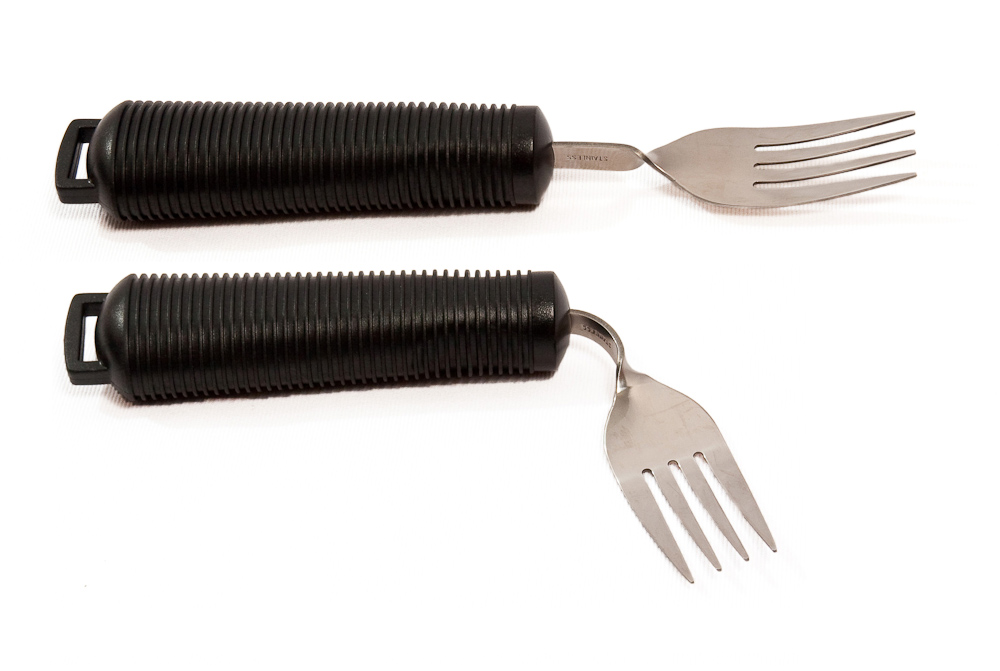
\includegraphics[width=5cm]{../figuras/talher.jpg}\\
			Fonte:\cite{vivere}
    
    \label{fig:talher}
  \end{center}
\end{figure}

A Figura \ref{fig:talher} mostra dois talheres que possuem cabos maiores para facilitar o manuseio, e um deles � ``dobrado'' para facilitar o posicionamento dos mesmos. Pacientes com quadros apresentados de Hemiplegia, Diplegia e algumas formas mistas podem se beneficiar com este tipo de talher.

}
\item{\acf{CAA}. Recursos eletr�nicos ou n�o para pessoas sem fala ou com limita��es dela (e.g., pranchas de comunica��o, vocalizadores, e softwares). A Figura \ref{fig:prancha} � um exemplo de prancha de comunica��o.

\begin{figure}[bth!]
  \begin{center}
    \caption{Exemplo de prancha de comunica��o}\vspace{.2cm}
			
      \centering
      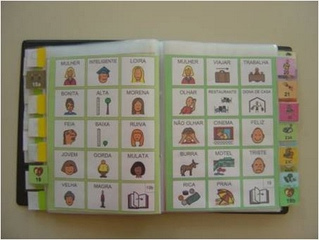
\includegraphics[width=5cm]{../figuras/prancha.jpg}\\
			Fonte:\cite{assistiva}
    
    \label{fig:prancha}
  \end{center}
\end{figure}

As pranchas de comunica��o exemplificadas na Figura \ref{fig:prancha} s�o meios de comunica��o para as pessoas com fala comprometida, isso pode ocorrer em todos os casos cl�nicos da \ac{PC}.

}
\item{Acessibilidade ao computador (e.g., teclados modificados, leitor de tela e ampliador de tela). A Figura \ref{fig:teclado} � um exemplo de teclado em modificado.
\vspace{-.5cm}
\begin{figure}[bth!]
  \begin{center}
    \caption{Exemplo de teclado em braile }\vspace{.2cm}
			
      \centering
      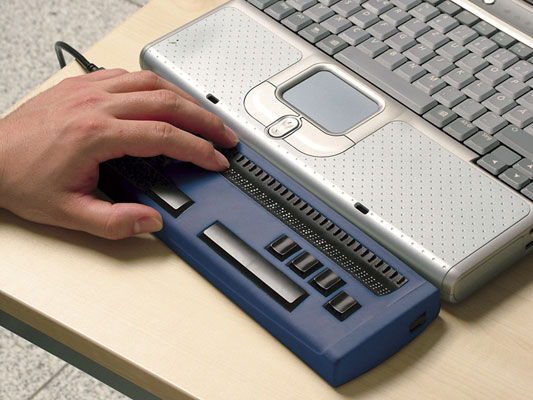
\includegraphics[width=4cm]{../figuras/teclado.jpg}\\
			Fonte:\cite{teclado}
    
    \label{fig:teclado}
  \end{center}
\end{figure}

A Figura \ref{fig:teclado} mostra que nos teclados modificados, a impress�o do que referencia cada tecla � na verdade um s�mbolo usado no alfabeto braile.

}
\item{Sistemas de controle de ambientes, que permitem que pessoas com dificuldades motoras controlem equipamentos a dist�ncia. A Figura \ref{fig:controle} � um exemplo de controle remoto para cegos.
\vspace{-.5cm}

\begin{figure}[bth!]
  \begin{center}
    \caption{Exemplo de controle assistivo}\vspace{.2cm}
			
      \centering
      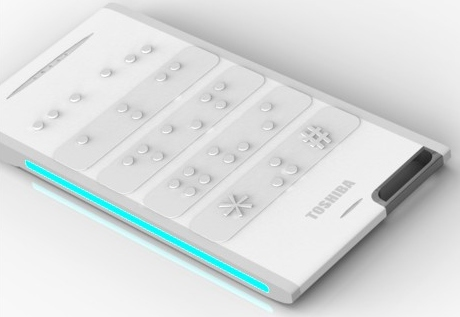
\includegraphics[width=4cm]{../figuras/controle.jpg}\\
			Fonte:\cite{controle}
    
    \label{fig:controle}
  \end{center}
\end{figure}
}
\vspace{-.5cm}
A Figura \ref{fig:controle} � um controle remoto que ao inv�s de possuir teclas com desenhos das fun��es e n�meros, os bot�es s�o representados em braile, para que os cegos possam manipular objetos a dist�ncia.

\item{Projetos Arquitet�nicos (e.g., cal�adas com guia para cegos e rampas de acesso). A Figura \ref{fig:rampa} � um exemplo de ramapa de acesso.

\begin{figure}[bth!]
  \begin{center}
    \caption{Exemplo de rampa de acesso}\vspace{.2cm}
			
      \centering
      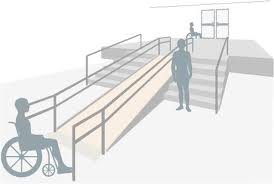
\includegraphics[width=4cm]{../figuras/rampa.jpg}\\
			Fonte:\cite{portal}
    
    \label{fig:rampa}
  \end{center}
\end{figure}

A Figura \ref{fig:rampa} representa uma rampa de acesso a cadeirantes, que torna poss�vel ao cadeirante o acesso a lugares mais elevados sem utilizar a ajuda de outras pessoas.

}
\item{�rteses e pr�teses, que permitem a troca ou ajuste de um membro. A Figura \ref{fig:protese} � um exemplo de pr�tese.
\vspace{-.5cm}
\begin{figure}[bth!]
  \begin{center}
    \caption{Exemplo de pr�tese}\vspace{.2cm}
			
      \centering
      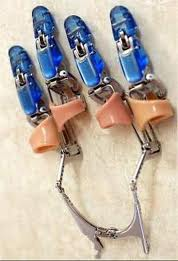
\includegraphics[width=3cm]{../figuras/protese.jpg}\\
			Fonte:\cite{protese}
    
    \label{fig:protese}
  \end{center}
\end{figure}
\vspace{-.5cm}
As pr�teses exemplificadas na Figura \ref{fig:protese}, ajudam as pessoas com membros danificados ou perdidos, a reabilita��o de movimentos.

}
\item{Equipamentos de aux�lio a postura (e.g., almofadas anat�micas e cintos). A Figura \ref{fig:cadeira} � um exemplo de cadeira de rodas com ajuste de postura.
\vspace{.5cm}
\begin{figure}[bth!]
  \begin{center}
    \caption{Exemplo de cadeira com regulagem de postura}\vspace{.2cm}
			
      \centering
      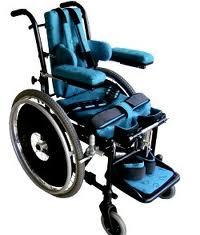
\includegraphics[width=4cm]{../figuras/cadeira.jpg}\\
			Fonte \cite{cadeira}
    
    \label{fig:cadeira}
  \end{center}
\end{figure}
}

Na Figura \ref{fig:cadeira} � poss�vel perceber o cinto na cadeira de rodas, que regulam a postura da pessoas do usu�rio.

\item{Equipamentos de mobilidade (e.g., cadeira de rodas motorizadas ou n�o e andadores). A Figura \ref{fig:cadeiramotorizada} representa um exemplo de cadeira de rodas motorizada.
\vspace{2cm}
\begin{figure}[bth!]
  \begin{center}
    \caption{Exemplo de cadeira de rodas motorizadas}
			
      \centering
      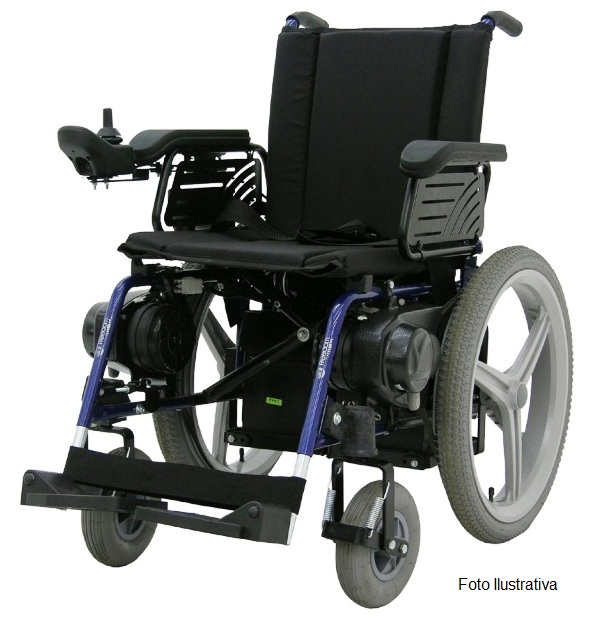
\includegraphics[width=3.5cm]{../figuras/cadeiramotorizada.jpg}\\
			Fonte: \cite{cinta}
    
    \label{fig:cadeiramotorizada}
  \end{center}
\end{figure}

Na Figura \ref{fig:cadeiramotorizada}, a cadeira possui um motor el�trico que faz com que a pessoa que a utiliza n�o necessite de grande esfor�o f�sico para moviment�-la.


}
\item{Aux�lio de surdos ou com audi��o parcial (e.g., aparelhos de surdez e telefones com teclado). A Figura \ref{fig:aparelhosurdez} � um exemplo de aparelho de surdez.
\vspace{-.5cm}
\begin{figure}[bth!]
  \begin{center}
    \caption{Exemplo de aparelho de surdez}
			
      \centering
      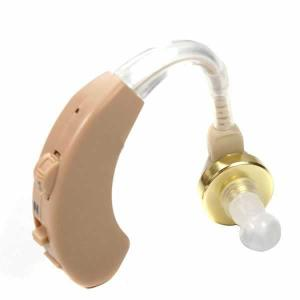
\includegraphics[width=3.5cm]{../figuras/aparelhosurdez.jpg}\\
			Fonte: \cite{surdez}
    
    \label{fig:aparelhosurdez}
  \end{center}
\end{figure}
}
\vspace{-.5cm}

Os aparelhos de surdez ilustrados pela Figura \ref{fig:aparelhosurdez} possibilitam que o �udio seja amplificado para que pessoas com defici�ncia auditiva parcial, possam escutar normalmente.

\item{Adapta��es a ve�culos. A Figura \ref{fig:carro} � um exemplo de carro adaptado a pessoas com defici�ncias f�sicas.
\begin{figure}[bth!]
  \begin{center}
    \caption{Exemplo de carro adaptado}\vspace{.2cm}
			
      \centering
      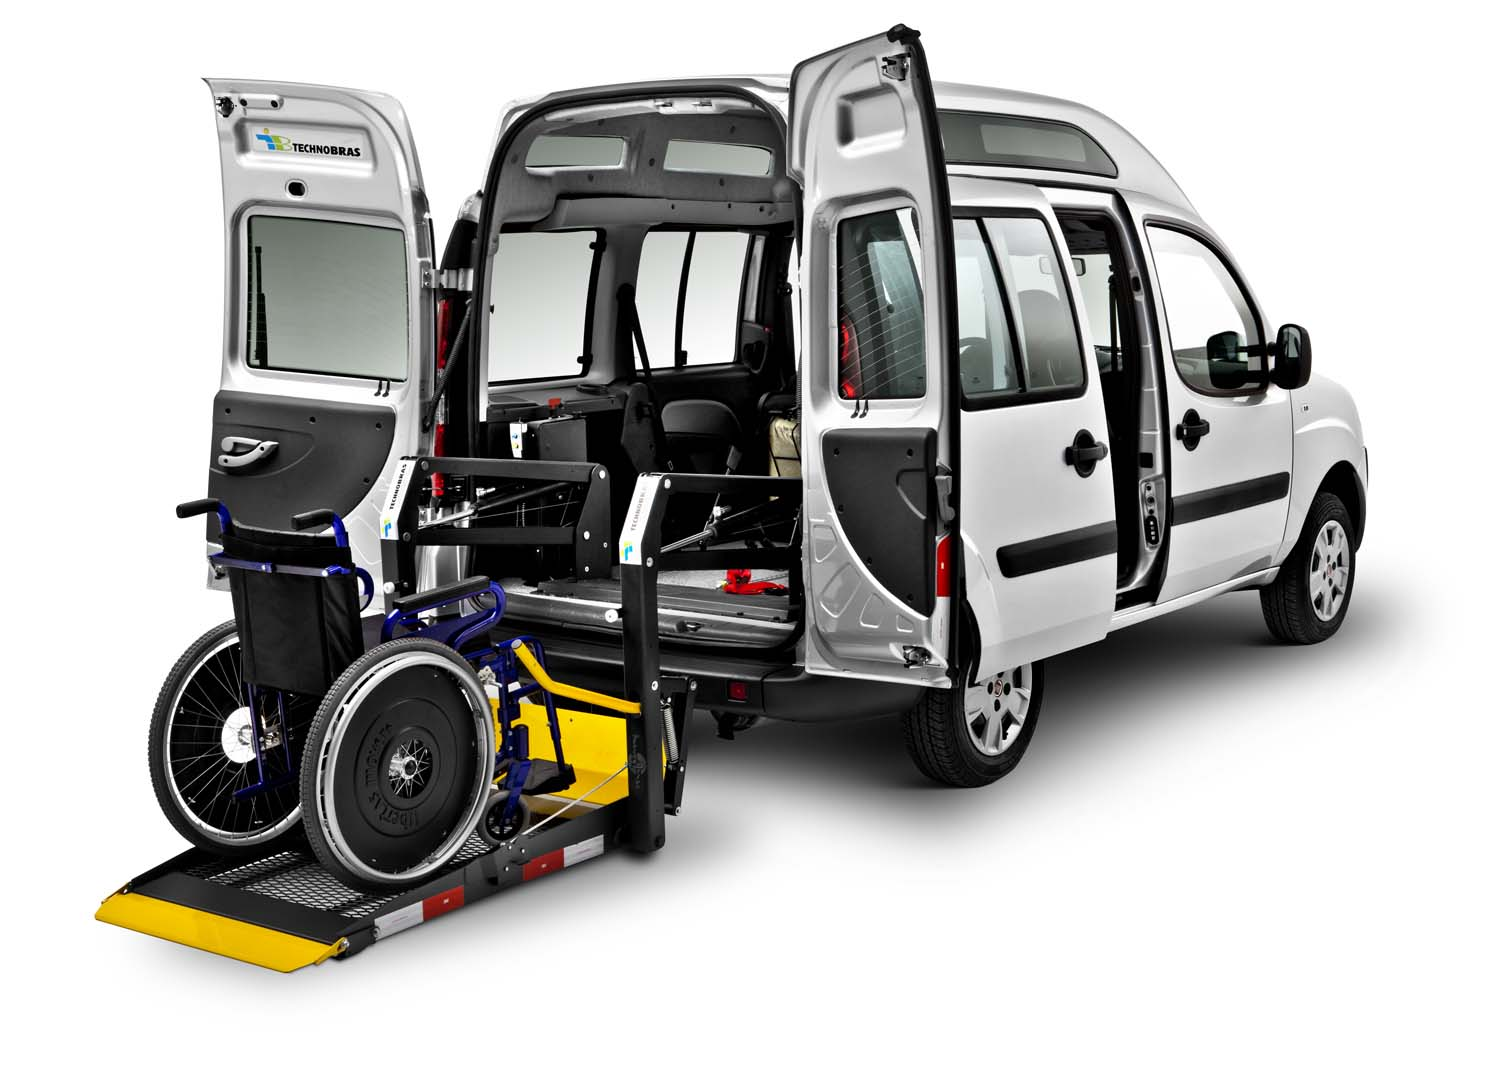
\includegraphics[width=4cm]{../figuras/carro.jpg}\\
			Fonte: \cite{fiat}
    
    \label{fig:carro}
  \end{center}
\end{figure}
}

A Figura \ref{fig:carro} � um exemplo de carro adaptado para pessoas com defici�ncia f�sica, possibilita que estas pessoas possam utilizar um ve�culo autonomamente.


\end{enumerate}


J� segundo a norma ISO 9999:2011(Anexo~\ref{iso9999}), a classifica��o das \ac{TA} se divide em categorias semelhante as diretrizes da \ac{ADA} por�m s�o mais espec�ficas. Para fins te�ricos, � utilizado no trabalho a classifica��o com base nas diretrizes da \ac{ADA} porque al�m da ISO 9999:2011 n�o incluir produtos e equipamentos usados exclusivamente por profissionais de sa�de e dispositivos implantados, a classifica��o \ac{ADA} apresenta um grupo de servi�os de \ac{TA} que promove o apoio � avalia��o da pessoa com defici�ncia, o desenvolvimento e personaliza��o de recursos, a integra��o da \ac{TA} com a��o e objetivos educacionais e de reabilita��o, e os apoios legais de concess�o \cite{corde}.


Uma pesquisa do \ac{W3C} \cite{wc} brasileiro aponta que das pessoas que usam aparelhos de \ac{TA}, 85\% � o computador o dispositivo mais usado, seguido do celular, {\it smarthphone} com 9\%, {\it tablet} com 2\%, e outros dispositivos com 4\%. Sendo cada vez mais necess�rio que existam op��es para esse tipo de p�blico dentro do acesso a informa��o.

A \ac{TA} faz parte da tecnologia, � a parte que auxilia a integra��o das pessoas que possuem algum tipo de defici�ncia. � uma �rea que envolve grandes por��es da popula��o, e que necessita de um cuidado especial, pois envolve al�m da pessoa com defici�ncia, as pessoas nos ambientes em que ela est� inserida.

\subsection{Legisla��o espec�fica de \acf{TA}}

Em rela��o a legisla��o de \ac{TA} alguns decretos s�o relevantes, entre eles a promulga��o do Decreto 3.298 
de 1999, que no artigo 19, fala do direito do cidad�o brasileiro com defici�ncia �s \ac{TA}. 
Nele consta que\cite{lima} (ver anexo {\ref{decreto1}}): 
\begin{quotation}
``Consideram-se ajudas t�cnicas, para os efeitos deste Decreto, os elementos que permitem 
compensar uma ou mais limita��es funcionais motoras, sensoriais ou mentais da pessoa 
portadora de defici�ncia, com o objetivo de permitir-lhe superar as barreiras da comunica��o e da 
mobilidade e de possibilitar sua plena inclus�o social. 
Par�grafo �nico. S�o ajudas t�cnicas:[...]elementos especiais para facilitar a comunica��o, a informa��o e a sinaliza��o para 
pessoa portadora de defici�ncia[...]``
\end{quotation}

O artigo 19 generaliza o termo Ajudas T�cnicas a todos os elementos que compensam limita��es do ser humano, por�m sem caracteriza��o ou classifica��o objetiva de tais ajudas. Tamb�m relevante, o decreto 5.296 de 2002, que d� prioridade de atendimento e estabelece normas gerais e crit�rios b�sicos para a promo��o da acessibilidade das pessoas com defici�ncia ou com 
mobilidade reduzida, possui um cap�tulo espec�fico sobre as ajudas t�cnicas no qual descreve 
v�rias inten��es governamentais na �rea da \ac{TA}, al�m de referir a constitui��o do 
\ac{CAT}. Neste decreto encontra-se que\cite{lima}: 
\begin{quotation}
``Consideram-se ajudas t�cnicas os produtos, instrumentos, equipamentos ou tecnologia 
adaptados ou especialmente projetados para melhorar a funcionalidade de pessoas portadoras de  
defici�ncia, com habilidade reduzida favorecendo autonomia pessoal, total ou assistida" .
\end{quotation}

No decreto 5.296\cite{cata} a legisla��o cita ao inv�s da compensa��o como no artigo 19, a autonomia total ou assistida das pessoas com defici�ncia. Embora esse Comit� leve a express�o ``Ajudas T�cnicas'' em sua 
denomina��o, tamb�m porque � a express�o prevista na legisla��o brasileira, 
os estudos desenvolvidos apontam e sugerem que as express�es 
``Tecnologia Assistiva'', ``Ajudas T�cnicas'' e ``Tecnologia de Apoio'', neste 
momento, continuem sendo entendidas como sin�nimos e que correspondam 
�s bases conceituais aprovadas pelo Comit�. Entretanto, estabelece a 
utiliza��o �nica da express�o ``Tecnologia Assistiva'' em seus documentos, 
como a mais apropriada, pelos seguintes motivos \apud{cata}{galvao}: 
\begin{itemize}
 
\item Por ser uma tend�ncia nacional j� firmada no meio acad�mico, nas 
organiza��es de pessoas com defici�ncia, em setores governamentais 
(Minist�rio MEC da Educa��o, Minist�rio da Ci�ncia e Tecnologia (MCT), Conselho Nacional de Desenvolvimento Cient�fico e Tecnol�gico CNPq), Institutos de Pesquisa (ITS Brasil) e no mercado de produtos; 
 
\item Pelo primeiro objetivo do Comit� de Ajudas T�cnicas, expl�cito no Artigo 
66 do Decreto 5296/2004, relativo � estrutura��o das diretrizes da �rea 
do conhecimento. A express�o Tecnologia Assistiva seria a mais 
compat�vel como a denomina��o de uma �rea de conhecimento, a ser 
oficialmente reconhecida; e
 
\item Por ser uma express�o bastante espec�fica ao conceito ao qual 
representa, diferentemente das express�es ``Ajudas T�cnicas'' e 
``Tecnologia de Apoio'', que s�o mais gen�ricas e tamb�m utilizadas para 
referirem-se a outros conceitos e realidades diferentes. 
\end{itemize}

Conforme votado e aprovado por unanimidade na quinta Reuni�o desse Comit�, al�m da determina��o de utiliza��o �nica da express�o Tecnologia Assistiva, foi decidido tamb�m que essa express�o seja utilizada no singular, por referir-se a uma �rea do conhecimento e sugere-se que se fa�am os poss�veis encaminhamentos para a revis�o da nomenclatura em 
instrumentos legais no pa�s. Este mesmo Comit� de Ajudas T�cnicas tamb�m aprovou, na sua terceira Reuni�o de abril de 2007, as bases conceituais que situam a Tecnologia Assistiva nos seguintes marcos \cite{cata,catb}: 

\begin{itemize}
\item �rea do Conhecimento;
\item Multidisciplinariedade;
\item Objetivos: promover a funcionalidade (atividade, participa��o) de 
pessoas com defici�ncia, mobilidade reduzida, ou idosas, visando sua 
autonomia, independ�ncia, qualidade de vida e inclus�o social; 
\item Composi��o: produtos, recursos, estrat�gias, pr�ticas, processos, 
m�todos e servi�os; e 
\item Ter presente os princ�pios do {\it Universal Design}\footnote{O conceito de Desenho Universal, ou ``{\it Universal Design}'', ou tamb�m chamado ``Desenho para todos'', � estudado a partir de alguns princ�pios tais como: equipara��o nas possibilidades de uso; flexibilidade no uso; uso simples e intuitivo; capta��o da informa��o; toler�ncia ao erro: m�nimo esfor�o f�sico; dimens�o e espa�o para uso e intera��o \cite{sepro}} e ITS BRASIL (Instituto de Tecnologia Social).

\end{itemize}

Apesar de uma iniciativa e uma legisla��o recente os assuntos acessibilidade e ajudas t�cnicas vem entrando no cotidiano dos brasileiros, pois h� uma cobran�a da parte governamental. Por�m, ainda existe uma defici�ncia em normas e na pr�pria legisla��o que regulamente as \ac{TA} principalmente na parte de classifica��o e exig�ncias.

\subsection{Iniciativas de \ac{TA}}
\label{iniciativas}

Existem v�rias iniciativas de \ac{TA} pelo mundo, como a  Funda��o SIDAR\cite{sidar} ({\it Seminario Iberoamericano sobre Diversidad y Accesibilidad en la Red}) que � uma institui��o de observa��o e recomenda��o na �rea da acessibilidade e inclus�o digital para os territ�rios ibero-americanos, a ATI\cite{ati} ({\it Assistive Technology Initiative}) na Universidade De George Mason na Virg�nia nos Estado Unidos, o INCNESI\cite{incnesi} (Iniciativa Nacional para os Cidad�os com Necessidades Especiais na Sociedade da Informa��o) que incentiva o uso de equipamentos para pessoas com defici�ncia em Portugal. 

Ainda no �mbito europeu, em 1999 foi organizado o Cons�rio \ac{EUSTAT} que desenvolveu um estudo entre 1997 e 1999, no contexto do Programa de Aplica��es Telem�ticas da Comiss�o Europeia, destinado a forma��o de usu�rios finais de \ac{TA}, envolvendo pessoas com defici�ncia ou idosos, seus familiares e profissionais assistentes pessoais, para que os mesmos pudessem fazer escolhas informadas, adequadas e respons�veis em rela��o a essas tecnologias. Esse estudo parte do princ�pio de que � fundamental a participa��o de usu�rio final como parceiro ativo na escolha das \ac{TA} que utiliza\cite{galvao}.

S�o parceiros do Cons�rcio \ac{EUSTAT} as seguintes organiza��es \cite{eustat}:

\begin{itemize}

\item SIVA {\it Servizio Informacione e Valutazione Ausili da Fondazione Dom Carlo Ghocchi Onlus}, da It�lia. Possui um centro de Inova��o e Transfer�ncia de Tecnologia, que incentiva projetos para autonomia de pessoas com defici�ncias;

\item CAPS  Centro de An�lise e Processamento de Sinais, do Instituto Superior T�cnico de Lisboa, Portugal;

\item \it{Association Nationale pour le Logement des personnes handicap�es}, da B�lgica;

\item \it{Groupement pour l�insertion des personnes handicap�es physiques}, da Fran�a;

\item \it{Danish Centre for Technical Aids for Rehabilitation and Education}, da Dinamarca; e

\item \it{Centro Studi Prisma}, da It�lia.

\end{itemize}

Os estudos que s�o parceiros do cons�rcio, s�o centros de refer�ncia em \ac{TA} na Europa, juntas s�o respons�veis por uma parte consider�vel de publica��es, dispositivos, sobre \ac{TA}. O Cons�rcio EUSTAT recomenda a classifica��o \ac{HEART} que prop�e tr�s grandes �reas de forma��o em 
rela��o �s \ac{TA}:
\begin{itemize} 
\item Componentes t�cnicos;
\item Componentes humanos; e
\item Componentes socioecon�micos.
\end{itemize}

Essa classifica��o tem ganhado for�a na atualidade, principalmente em decorr�ncia do paradigma inclusivo, o qual desloca as limita��es de funcionalidade e possibilidades de participa��o do �mbito restrito � defici�ncia em si, para situ�-las a partir das barreiras impostas pelo ambiente f�sico e social\cite{rodrigues}. Como n�o foi encontrado uma padroniza��o mundial para a defini��o de \ac{TA} as diferentes iniciativas encontradas se relacionam na tabela \ref{tabeladois}.

\begin{table}[bth!]
\centering
\scriptsize
\caption{Tabela com as diferen�as de Iniciativas de \ac{TA} encontradas.}\vspace{.2cm}
 \begin{tabular}{|p{2cm} |  p{3.9cm} | p{3cm} | p{4cm}| }
    \hline
    Pa�s & Termo Utilizado (Tradu��o) & Classifica��o & Defini��o \\ \hline
    Brasil & Tecnologia Assistiva, Ajudas T�cnicas &Ca\-te\-go\-ri\-as relativas aos e\-qui\-pa\-men\-tos & Melhorar as pessoas com defici�ncia e mobilidade re\-du\-zi\-da \\ \hline
    EUTSTAT & Ajudas T�cnicas e Tecnologia de Apoio & Classifica��o por componentes& Compensar as pessoas com defici�ncia e idosas \\ \hline
    ADA & {\it Assistive Technology} (Tecnologia Assistiva) & Trata as situa��es & Ajudas aos indiv�duos com defici�ncia em situa��es es\-pe\-c�\-fi\-cas \\ \hline	
		\end{tabular}
    \label{tabeladois}
		\\Fonte: o pr�prio autor.

\end{table}

A tabela {\ref{tabeladois}} mostra as diferen�as das tr�s iniciativas mais relevantes encontradas. Apesar da mudan�a de termos, as iniciativas n�o possuem grandes diferen�as entre si. A classifica��o da \ac{TA} � o �nico fator que diferencia nas iniciativas. Por�m, a relev�ncia da mudan�a � pequena, em rela��o a as ajudas �s pessoas com defici�ncia.


\section{Comunica��o Alternativa Ampliada (CAA)}

Na \ac{TA}, como mencionado anteriormente na se��o {\ref{Tecnologia Assistiva}} se divide em algumas classifica��es, dentro delas temos a \ac{CAA}, que � linha de pesquisa adotada neste trabalho. A \ac{CAA} abrange qualquer meio de comunica��o que suplemente ou substitua os m�todos naturais de fala ou escrita. � um meio que auxilia a comunica��o de um indiv�duo com outras pessoas. Os sistemas de \ac{CAA} podem ser divididos em pictoriais\footnote{Os sistemas pictoriais representam os referentes por analogia f�sica e n�o por conven��o arbitr�ria, o que lhes confere iconicidade e clareza denotativa, sendo bem compreendidos, aprendidos e lembrados por crian�as, estrangeiros e c�rebro-lesados. Contudo, o universo de significados que podem representar restringe-se ao imagin�vel \cite{fernando}.} e simb�licos\footnote{Os sistemas simb�licos representam referentes por conven��es arbitr�rias, usando regras de recombina��o e sintaxe espec�fica, o que resulta em opacidade denotativa, mas lhes permite representar virtualmente qualquer conceito, imagin�vel ou n�o \cite{fernando}.} podendo ser de alta tecnologia (e.g., sistemas computadorizados, e softwares especiais) e baixa tecnologia (e.g., simples, e n�o el�tricos) \cite{leydi}.

A \ac{CAA} � definida como uma maneira alternativa � comunica��o oral e escrita que compreende o uso de gestos, sinais manuais, express�es faciais, pranchas com s�mbolos pictogr�ficos, pranchas de alfabeto, comunicadores de voz gravada ou sintetizada at� sistemas sofisticados de computador \apud{glennen}{correia}. Inicialmente eram utilizados sistemas sem tecnologia, recorrendo apenas ao corpo humano, como a linguagem por sinais (e.g., libras) passando pelos sistemas anal�gicos ou de baixa tecnologia (e.g., cart�es e livros com s�mbolos e imagens) at� sistemas baseados em recursos computacionais (e.g., vocalizadores, e softwares para computador com s�ntese de voz) \apud{worthy}{correia}.

O trabalho da \ac{CAA} engloba uma s�rie de s�mbolos, recursos, estrat�gias e t�cnicas para auxiliar o desenvolvimento de uma comunica��o complementar. Os s�mbolos s�o as representa��es visuais, auditivas ou t�teis de um conceito; os recursos s�o os objetos ou equipamentos utilizados para transmitir as mensagens que podem ser pranchas de comunica��o, os comunicadores ou o computador; as t�cnicas s�o as formas como as mensagens s�o transmitidas e as estrat�gias referem-se ao modo como os recursos da \ac{CA} s�o utilizados \apud{king}{pelosi2}.

Como o foco deste trabalho � encontrar uma solu��o alternativa a pessoas que possuem defici�ncia na fala, em conjunto com defici�ncia motora (quadros tabela cl�nicos), a \ac{CAA} � a abordagem encontrada que melhor se encaixa neste contexto. Pois a \ac{CAA} utiliza estrat�gias e t�cnicas para o desenvolvimento de uma comunica��o complementar, que auxiliam a suplementa��o ou substitui��o da forma natural de comunica��o.


\section{Considera��es do Cap�tulo}

Com a pesquisa realizada no cap�tulo {\ref{cap:introducao}}, fica evidenciado que pessoas com necessidades especiais, precisam de recursos que supram ou compensem suas defici�ncias para que possam ser inseridas na sociedade. Apesar de uma por��o consider�vel da popula��o mundial possuir algum tipo de defici�ncia, os estudos e legisla��o sobre a \ac{TA} s�o consideravelmente recentes.
	
Al�m disso, vale ressaltar a import�ncia de que se desenvolva mais solu��es de \ac{TA}, principalmente acess�veis, e que os desenvolvedores, se preocupem com o ambiente em que esta pessoa est� inserida e as pessoas com as quais ela ir� interagir. Foram necess�rios conhecimentos sobre \ac{TA}, \ac{CAA} e acessibilidade para que se entenda o foco deste trabalho que visa encontrar uma solu��o alternativa de \ac{CAA} para pessoas que possuem \ac{PC} que apresentam defici�ncia motora e de fala.
	
Este trabalho se enquadra na Lei no 10.098, de dezembro de 2000 que estabelece crit�rios como o artigo 17 que garante direito de comunica��o e express�o por mecanismos, ou alternativas t�cnicas. Al�m disso, se enquadra tamb�m, no Decreto 5296/2004, Artigo 66 do Comit� de Ajudas T�cnicas, no qual estabelece o termo \acf{TA} como a denomina��o mais compat�vel ao tema.

O trabalho tamb�m pode ser classificado nas diretrizes da \ac{ADA} como um trabalho no contexto de \acf{CAA}. J� na norma ISO 9999:2011 na subcategoria, Produtos de Apoio para Treino de Comunica��o Alternativa e Aumentativa, c�digo 05 06 27, categoria Produtos de apoio para treino de comunica��o com imagens e desenhos.

\chapter{Cap\'itulo 2}


\chapter{Proposta para caracterização de tráfego}
\label{cap3}

Para realizar a caracterização de tráfego em uma rede é necessário coletar/medir o tráfego para posterior análise, conforme descrito na Seção~\ref{cap2:caracterizacao}.
%
Na fase de medição de tráfego é possível aplicar ferramentas existentes (\textit{e.g., } \texttt{Tcpdump}, Bro, \texttt{ping}) para recolher os dados que serão utilizados na fase de análise.
%
Contudo, por serem ferramentas amplamente difundidas e com propósito geral, estas geram dados genéricos (\textit{e.g.,} pacote inteiro), que não captam apenas os aspectos desejados para posterior análise.
%
Sendo assim, a criação de uma ferramenta de monitoramento possibilita recolher apenas os dados pertinentes a análise em questão.

Contudo, ao tratar-se da caracterização envolvendo um software complexo como o OpenStack, é necessário conhecer pelo menos a arquitetura de funcionamento dos serviços envolvidos no processo de caracterização de tráfego, conforme apresentado na Seção \ref{cap3:openstack_detalhes}.
%
Pois conhecendo o funcionamento dos serviços do OpenStack é possível entender como capturar o tráfego de interesse, quais são os seus aspectos analisáveis, e quais as melhores abordagens a adotar (Seção \ref{cap3:ambiente}).
%
Tendo estas informações em mãos, pode-se definir os requisitos para a criação do sistema de monitoramento, conforme exibido na Seção \ref{cap3:requisitos}.
%
A partir dos requisitos e das observações sobre o ambiente do OpenStack, na Seção \ref{cap3:monitoramento} é estabelecida a arquitetura do sistema de monitoramento.
%
Algumas informações geradas pelo sistema de monitoramento podem ser aplicadas diretamente para entender o tráfego, permitindo sua análise em tempo real. 
%
Contudo, certas informações necessitam de análises minuciosas, cujo processo, por exemplo, precisa que sejam feitas comparações com outras informações coletadas a fim de gerar dados significativos.
%
A fase seguinte à coleta realizada pelo sistema de monitoramento é a de análise de tráfego, cuja abordagem para o problema proposto é definida na Seção \ref{cap3:analise}.
%
Sendo explicado o que é feito com os dados coletados, e qual o tipo de informação resultante da análise.
%
Por fim, define-se na Seção \ref{cap3:experimento} como será aplicado o sistema de monitoramento, na qual explica-se os cenários de aplicação e os detalhes referentes à realização dos experimentos.

\section{Funcionamento do OpenStack}
\label{cap3:openstack_detalhes}

Conforme apresentado na Seção \ref{cap2:openstack}, a instalação do OpenStack pode distribuir os serviços entre vários hosts. 
%
Segundo a arquitetura sugerida na documentação oficial \cite{openstack:newton}, são atribuídas responsabilidades específicas para cada host da nuvem, classificados em: armazenamento, computação, controle, e de rede.
%
Estas categorias são definidas conforme os serviços executados no host, e dependendo do tamanho da nuvem, um host pode pertencer a múltiplas categorias, sendo responsável por controle e armazenamento, por exemplo.
%
No caso de nuvens maiores esta centralização é evitada por questões de desempenho.
%
A Figura \ref{fig:openstack_instalacao_servicos} apresenta uma arquitetura de instalação conceitual do OpenStack, na qual um dos hosts opera como nó de controle da nuvem e nó de rede simultaneamente.
%
Esta nomenclatura segue a utilizada na documentação do OpenStack, na qual ao referenciar-se às atribuições do host, coloca-se a palavra nó na frente, referenciando um host com serviços relacionados ao Neutron, por exemplo, como nó de rede.

\vspace{-0.3cm}
\begin{figure}[!htb]
	\centering
	\caption{Arquitetura conceitual de instalação de componentes do OpenStack}
    \vspace{-0.3cm}
	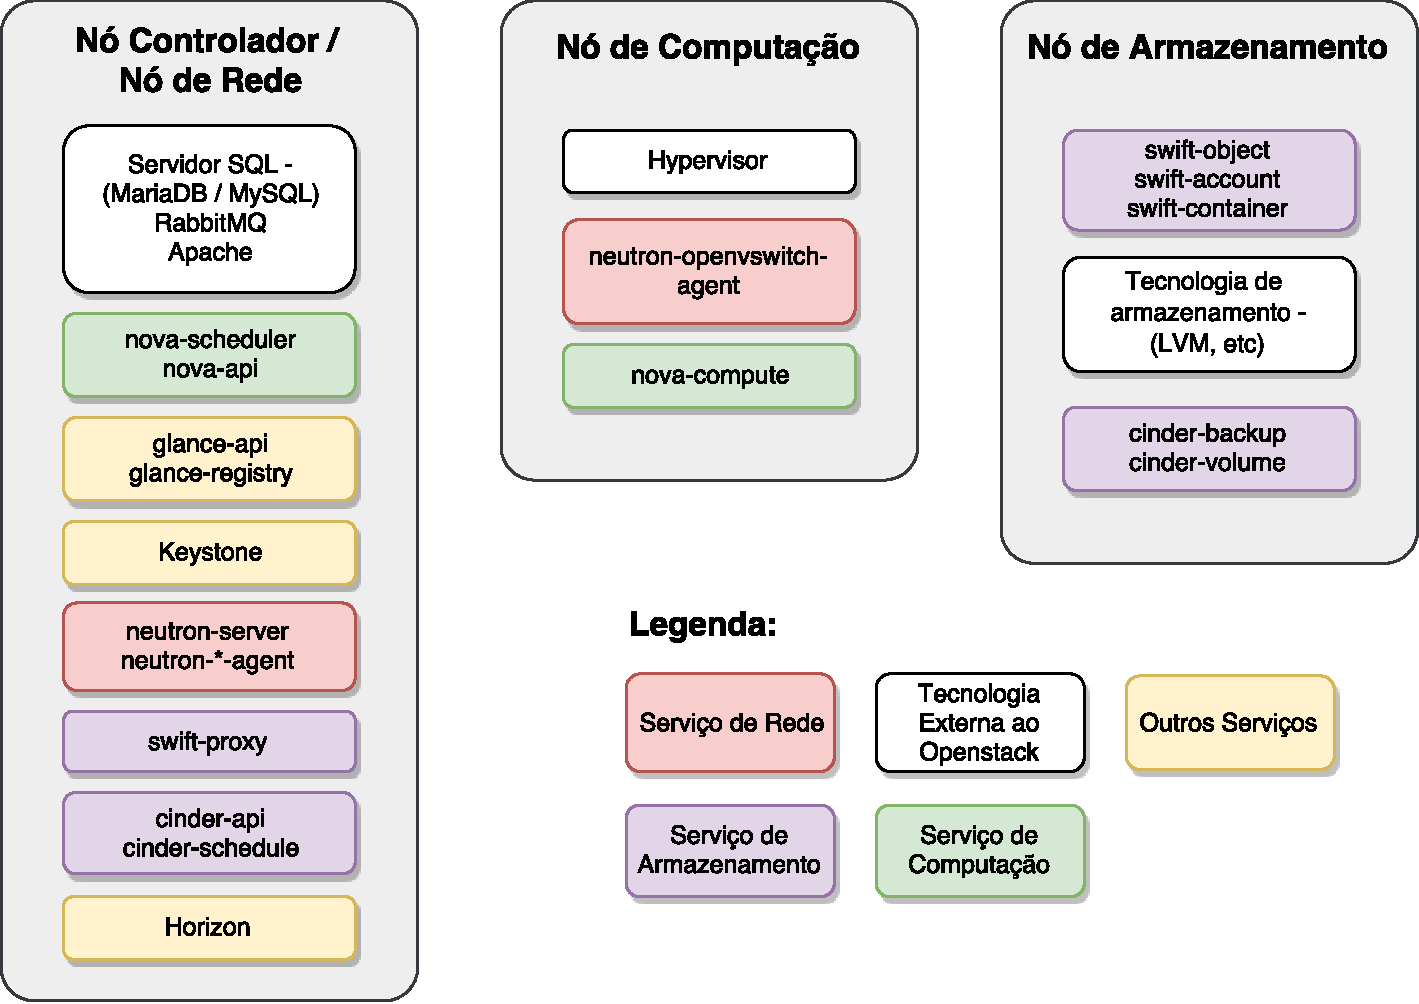
\includegraphics[width=.75\textwidth]{img/openstack_arquitetura_instalacao.pdf}
	\label{fig:openstack_instalacao_servicos}\\
    \vspace{-0.3cm}
	Fonte: O próprio autor.
\end{figure}

\vspace{-0.5cm}
Para explicitar melhor o papel de cada uma das categorias de host no tráfego de controle, esta seção apresenta brevemente como funcionam alguns serviços que executam nestes hosts, com foco na suas respectivas arquiteturas.
%
Os serviços apresentados nesta seção são os considerados no monitoramento e posterior análise do tráfego, conforme definido na Tabela~\ref{tab:openstack_service_list}, com exceção do Horizon, que é basicamente uma interface web que acessa as \acp{api} dos outros serviços, e não será abordado na explicação.
%
Esta limitação de serviços abordados visa simplificar o processo de caracterização, e segue a recomendação de serviços populares em uma instalação do OpenStack, segundo \cite{openstack:about}.



Nem todos os serviços do OpenStack têm a mesma complexidade, e neste sentido, alguns serviços como Nova e Neutron destacam-se pela complexidade.
%
Portanto, nesta seção alguns serviços mais complexos são abordados em mais detalhes do que outros com arquitetura simples (\textit{e.g.,} Keystone, Swift).
%
Além dos serviços, também é apresentada a ferramenta RabbitMQ, que possui papel importante na comunicação entre componentes pertencentes a certos serviços.
%
Esta seção inicia com o Nova, um dos serviços principais no OpenStack, que gerencia o ciclo de vida das \acp{vm} e se relaciona com vários dos serviços do OpenStack para dispor suas funcionalidades (Figura \ref{fig:openstack_service_architecture}).

\subsection{Nova}

O Nova é o serviço de computação do OpenStack, o qual gerencia os nós de computação existentes na nuvem, controlando os \textit{hypervisors} instalados nestes nós, e consequentemente, as \acp{vm} em execução. 
%
Versões anteriores do OpenStack também incluem componentes relacionados à configuração de rede no Nova (\texttt{nova-network}), que disponibiliza um modelo de gerenciamento de rede mais limitado quando comparado ao Neutron, e portanto foi descontinuado.
%
Segundo \citeonline{redhat:components}, as versão recentes do Nova utilizam uma arquitetura que divide-se em diversos componentes, conforme ilustrado na Figura \ref{fig:nova_architecture}.

\begin{figure}[!htb]
	\centering
	\caption{Arquitetura dos componentes pertencentes ao serviço Nova}
    \vspace{-0.3cm}
	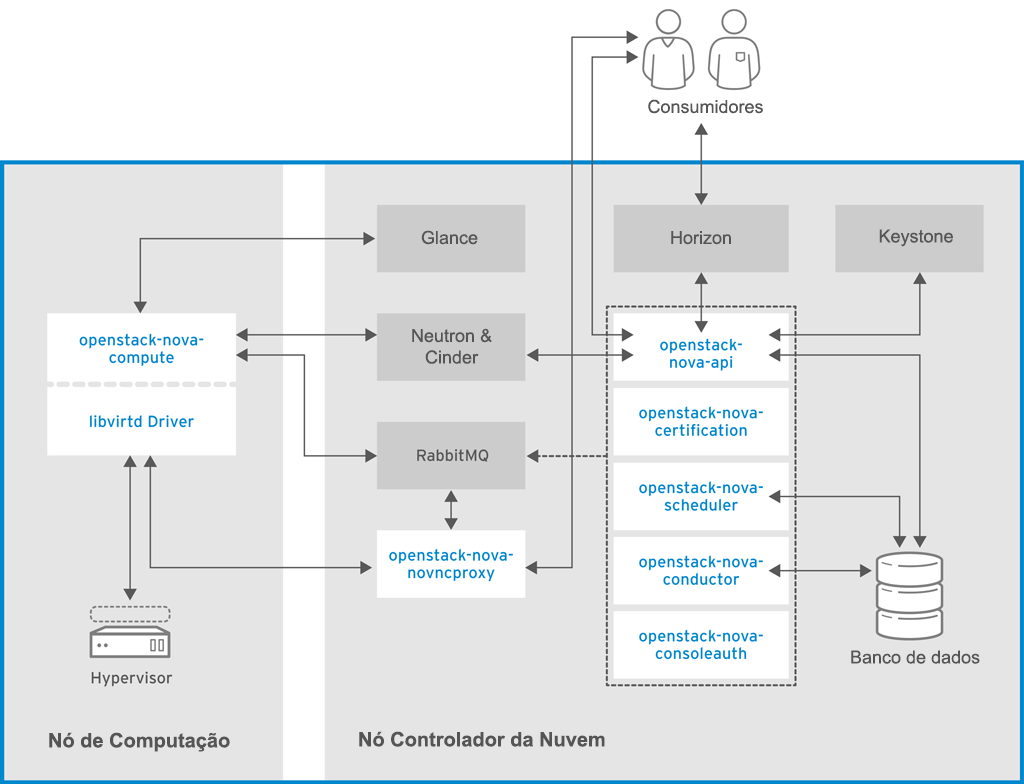
\includegraphics[width=.8\textwidth]{img/nova_arquitetura.png}
	\label{fig:nova_architecture}\\
	Fonte: Adaptado de \cite{redhat:components}.
\end{figure}

Apesar dos vários componentes pertencentes ao serviço Nova (Figura \ref{fig:nova_architecture}), este trabalho foca em alguns componentes principais: \ac{api}, escalonamento, computação, banco de dados, e \textit{message broker} (AMQP Server).

Conforme apresentado na Seção \ref{cap2:openstack}, a \ac{api} do Nova (\texttt{nova-api}) é responsável por disponibilizar acesso e tratar requisições para o serviço Nova.
%
O \texttt{nova-api} em sua essência é um \textit{Web Service} implementado sobre o protocolo REST, e gerencia autorização e funções básicas de controle, na qual implementa modelos de API compatíveis como o da Amazon e Rackspace.
%
Existem diferentes versões da REST \ac{api} do Nova, que introduzem novas funcionalidades ou padronizações, o OpenStack Newton por exemplo, que é a versão que este TCC irá trabalhar, tem a REST \ac{api} do Nova na versão 2.38 \cite{openstack:newton:api}.
%
Toda requisição recebida pelo \texttt{nova-api} é avaliada para verificar se os recursos referenciados na requisição estão disponíveis, e caso estiverem disponíveis, a requisição é enviada ao \textit{message broker}, que é um servidor \acf{amqp}, e disponibiliza a mensagem para os recursos referenciados acessarem \cite{openstack:nova}.
%
O \textit{message broker} é um \textit{middleware} com o protocolo \ac{amqp} utilizado para comunicação interna entre componentes de certos serviços, que no caso do Nova por exemplo, se aplica aos componentes \texttt{nova-scheduler} e \texttt{nova-compute}, e também intermedeia o acesso ao banco de dados pelo \texttt{nova-compute}.

Durante a troca de mensagens, o \textit{message broker} também atualiza o banco de dados do Nova, que mantém informações sobre o estado corrente da nuvem, como por exemplo, o números de \acp{vm} executando em cada nó de computação da nuvem \cite{redhat:components}.
%
Este banco de dados é implementado em MySQL e é acessível pelos componentes do Nova, o qual centraliza as informações que os componentes necessitam durante sua execução.
%
Após receber a mensagem contendo o pedido de \ac{vm} pelo \textit{message broker}, o componente responsável pelo escalonamento, chamado \texttt{nova-scheduler} define qual nó de computação hospedará uma nova instância de \ac{vm}.
%
Para definir o nó de computação é consultado o banco de dados do Nova, que contém informações aplicáveis no processo de filtragem para encontrar um nó de computação disponível para hospedar a \ac{vm}.
%
Neste sentido, é possível fornecer pesos para as métricas, ajudando na escolha do nó de computação, como também é possível deixar a escolha aleatória entre os nós de computação filtrados no processo, que correspondem aos nós de computação podendo hospedar aquela \ac{vm} \cite{openstack:nova}.

No caso de uma nuvem de pequeno porte, os componentes do Nova exibidos até aqui executam em um mesmo nó de controle, pois não necessitam de grande quantidade de processamento.
%
Em contraste, o componente \texttt{nova-compute} executa em cada host que contém um \textit{hypervisor}, ou seja, um nó de computação, e é responsável por gerenciá-los.
%
Como todos os outros componentes do Nova que usam \ac{amqp}, o \texttt{nova-compute} em execução verifica periodicamente por tarefas enfileiradas para ele, e realiza-as conforme solicitado (\textit{e.g.,} criar instância, finalizar instância, ler saída do \textit{console}).
%
Se outros serviços que dispõem funcionalidades extras às \acp{vm} estiverem instalados (\textit{e.g.,} Cinder, Glance, Neutron), cada \texttt{nova-compute} realiza a comunicação direta com estes serviços.


\subsection{Cinder}

Para disponibilizar armazenamento persistente às \acp{vm}, o serviço Cinder permite acoplar volumes/blocos de armazenamento nas \acp{vm} em execução.
%
Além de disponibilizar armazenamento para \acp{vm}, o Cinder também fornece a habilidade de criar \textit{snapshots} dos volumes de armazenamento, que copia o conteúdo do volume, e possibilita gerar novos volumes contendo os dados deste \textit{snapshot}.
%
Mesmo sendo mais simples que o Nova, o Cinder também emprega múltiplos componentes para realizar suas funções, que podem ser distribuídos entre diferentes hosts.
%
Alguns componentes com comportamento similar aos componentes do Nova estão presentes: escalonador, banco de dados, \ac{api} e \textit{message broker}; em que difere-se nos componentes responsáveis pelo armazenamento: \texttt{cinder-backup} e \texttt{cinder-volume}.

O papel do \texttt{cinder-api}, componente que gerencia a \ac{api} do Cinder, é disponibilizar uma interface REST para que os outros serviços do OpenStack, como o Nova, acessem suas funcionalidades \cite{redhat:components}.
%
A REST \ac{api} do Cinder encontra-se na v3.15 no OpenStack Newton \cite{openstack:newton:api}.
%
Após recebido o pedido pelo \texttt{cinder-api}, ele é enviado ao \textit{middleware} responsável pela comunicação entre os componentes, baseado no protocolo \ac{amqp}, e que não necessita ser de uso exclusivo do Cinder.

O banco de dados, baseado em MySQL, tem propósito similar ao banco de dados no Nova: compartilhar informações relacionadas ao estado atual do serviço para os componentes, na qual também pode usar o mesmo servidor de banco de dados.
%
O escalonador \texttt{cinder-scheduler} decide onde armazenar volumes e backups criados, cuja funcionalidade é disponibilizada pelos componentes \texttt{cinder-volume} e \texttt{cinder-backup}, que podem ser hospedados em múltiplos hosts, servindo como nós de armazenamento.
%
Segundo \citeonline{redhat:components}, estes dois componentes podem usar várias soluções de armazenamento (\textit{e.g.,} Ceph, LVM, NFS), e em especial o \texttt{cinder-backup} é capaz de armazenar seus backups no Serviço de armazenamento Swift.

\subsection{Swift}

O Swift é outro serviço do OpenStack responsável pelo armazenamento, mas com o foco em armazenar dados estáticos de grande volume (\textit{e.g.,} vídeos, imagens, imagens de \ac{vm}).
%
O acesso aos dados é feito com o um pedido HTTP (\texttt{Get, Put, Delete}) para o \texttt{swift-proxy}, que é o componente do Swift responsável pela \ac{api}, e autenticação no serviço, que no OpenStack Newton encontra-se na v1 \cite{openstack:newton:api}.
%
Ao receber uma requisição é consultado a localização do objeto nos outros componentes (\texttt{swift-account}, e \texttt{swift-container}, respectivamente), roteando então a requisição de acordo com as informações consultadas, conforme ilustrado na Figura \ref{fig:swift_components}.

O Swift tem dois componentes que gerenciam acesso a listagem de informações: o \texttt{swift-account}, que gerencia a lista de contêineres de armazenamento no banco de dados, e o \texttt{swift-container}, cuja tarefa é gerenciar a lista de objetos contidos nos contêineres, também armazenado no banco de dados.
%
Para gerenciar os objetos armazenados, o componente \texttt{swift-object} armazena, recupera e exclui objetos conforme requisitado \cite{openstack:swift}.
%
A parte de autenticação do \texttt{swift-proxy} comunica-se com o serviço Keystone, que fornece uma \ac{api} que centraliza o processo de autenticação do OpenStack.

\begin{figure}[!htb]
	\centering
	\caption{Arquitetura dos componentes pertencentes ao serviço Swift}
    \vspace{-0.3cm}
	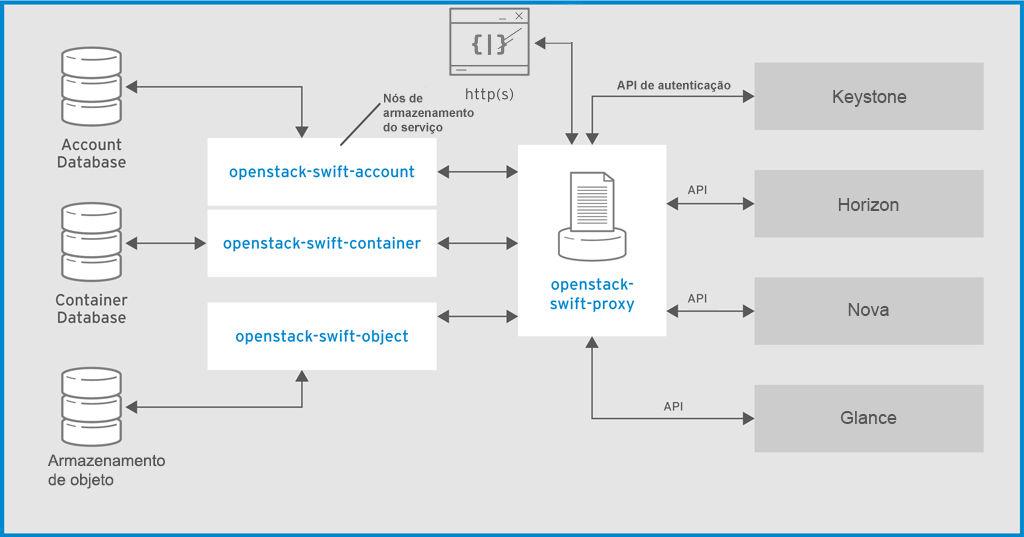
\includegraphics[width=.8\textwidth]{img/swift_arquitetura.png}
	\label{fig:swift_components}\\
	Fonte: Adaptado de \cite{redhat:components}.
\end{figure}

\subsection{Keystone}

O serviço Keystone fornece autenticação e autorização aos serviços do Openstack. 
%
Este serviço possibilita a autenticação através de múltiplos mecanismos, como por exemplo, credencial com usuário e senha, ou através de \textit{tokens} \cite{redhat:components}.
%
Desta maneira, é possível combinar estes mecanismos no uso do Keystone, no qual um pedido de autenticação é validado através de usuário e senha, e então, o serviço pode retornar um \textit{token} ao solicitante, que é utilizado para a autenticação posteriormente \cite{openstack:keystone}.

A arquitetura de funcionamento do Keystone é relativamente simples, possuindo apenas um componente principal, que é responsável pela \ac{api} do serviço, e encontra-se na v3 no OpenStack Newton.
%
A \ac{api} do Keystone armazena as identidades, autorizações, catálogos de serviços e \textit{tokens} no MySQL (MariaDB) por padrão, podendo-se adicionar outras tecnologias para cuidar de partes específicas do serviços. 
%
Neste sentido, a tecnologia \ac{ldap} pode ser empregada no gerenciamento de autenticações e \textit{memcache} ou \textit{Redis} para gerenciar a persistência dos \textit{tokens} \cite{redhat:components}.
%
Após autenticado o usuário (consumidor ou administrador), ele é capaz de acessar o catálogo fornecido pelo Keystone, cuja funcionalidade é armazenar os serviços em funcionamento no Openstack, e informar ao usuário quais recursos ele pode acessar.


\subsection{Glance}

O serviço Glance funciona como um registro de imagens de \acp{vm} acessível pelos consumidores da nuvem. 
%
É possível que os consumidores adicionem novas imagens, desde que estas sejam em um dos formatos aceitos pelo serviço, que segundo \citeonline{redhat:components}, inclui \texttt{iso}, \acp{vm} do VirtualBox (\texttt{vdi}), VMware (\texttt{vmdk}) e Amazon EC2 (\texttt{ami}).
%
Outra alternativa é gerar um \textit{snapshot} a partir de uma das \acp{vm} do consumidor, que pode servir como \textit{backup} ou imagem para iniciar outras \acp{vm}.

Em relação à sua arquitetura, o Glance é dividido nos seguintes componentes principais \cite{openstack:glance}: \texttt{glance-api}, \texttt{glance-registry}, repositório de armazenamento e banco de dados (MySQL/MariaDB).
%
A \ac{api} do Glance (\texttt{glance-api}) gerencia todos os pedidos para recuperação e armazenamento de imagens, que no OpenStack Newton tem a \ac{api} v2 \cite{openstack:newton:api}.
%
Enquanto os pedidos são processados, o componente \texttt{glance-registry} acessa o banco de dados instalado para buscar informações da imagem em questão (\textit{e.g.,} metadados da imagem, local de armazenamento).
%
As imagens registradas neste serviço podem ser armazenadas no serviço Swift ou através de outras tecnologias como RADOS Block Service, VMware datastore, HTTP, ou até como arquivo no próprio sistema de arquivos do host do Glance.


\subsection{Neutron}

Conforme apresentado na Seção \ref{cap2:openstack_network_architecture}, uma das funcionalidades do serviço Neutron é fornecer rede às \acp{vm} dos consumidores, incluindo a possibilidade de configurar a rede em questão, sub-redes e os seus roteadores \cite{redhat:components}.
%
Outras funcionalidades adicionais também podem ser oferecidas para a rede criada em um \textit{project}/\textit{tenant}, como DHCP (\texttt{neutron-dhcp-agent}), \textit{Firewall} ou \acp{vpn}.

\begin{sloppypar}
Comparado com os outros serviços do OpenStack, o Neutron é um dos mais complexos, podendo envolver diversas tecnologias de rede e possibilidades de configuração \cite{denton:2016:neutron}.
%
No geral, o Neutron tem os seguintes componentes: \textit{Network agents}, que inclui os componentes \texttt{neutron-dhcp-agent}, \texttt{neutron-openvswitch-agent} e \texttt{neutron-l3-agent}; \texttt{neutron-server} e \textit{message broker} \cite{openstack:neutron}.
%
Os \textit{Network agents} executam em todos os hosts de uma nuvem OpenStack, e são responsável por cuidar, por exemplo, da configuração das \acp{vm} contidas no host e também de serviços e \textit{plugins} em execução no Neutron, como o Open vSwitch (\texttt{neutron-openvswitch-agent}).
%
O Open vSwitch é uma das tecnologias que pode ser empregada na virtualização das interfaces de rede físicas dos hosts, e permite criar \acp{vlan} para isolar o tráfego de cada rede.
%
Assim, é possível que o tráfego de dois domínios diferentes trafeguem no mesmo meio físico com isolamento.
\end{sloppypar}

O componente \texttt{neutron-ml2} (Modular Layer 2) é obrigatório no Neutron, e controla a Camada 2 da rede, ou seja, encaminha pacote apenas dentro das redes criadas pelos consumidores.
%
A nível estrutural, o \texttt{neutron-ml2} funciona como um \textit{framework} que possibilita a criação de \textit{plugins} que relacionam-se com a Camada 2 da rede, como o TaaS (\textit{Tap-as-a-Service})\footnote{\url{https://github.com/openstack/tap-as-a-service}}, por exemplo.
%
O TaaS possibilita a criação de espelhamentos de portas das redes dos consumidores da nuvem, que tornam-se acessíveis através de portas virtuais criadas pelo TaaS no Open vSwitch, cuja aplicação inclui, por exemplo, o monitoramento do tráfego com um \ac{ids}.
%
Para fornecer acesso à rede externa um \textit{L3 Network agent} (\texttt{neutron-l3-agent}) deve executar no nó de rede da nuvem, e responsabilizar-se pelo roteamento dos pacotes para fora da rede do consumidor, que corresponde à função do roteador virtual inserido pelo consumidor na sua rede \cite{redhat:components}.
%
O agente DHCP (\texttt{neutron-dhcp-agent}) é outro agente que executa no nó de rede, e fornece o serviço de DHCP para as redes dos consumidores.

Por fim, o componente \texttt{neutron-server} é responsável pela \ac{api} do serviço, que age similar aos outros serviços, na qual envia as mensagens para o \textit{message broker}, que encaminha-as para os outros agentes e \textit{plugins} do Neutron.
%
Através da sua \ac{api} os consumidores definem as configurações das suas redes, e o administradores definem as tecnologias de redes empregadas nos serviços do Neutron \cite{denton:2016:neutron}.
%
A \ac{api} do Neutron encontra-se na v2 atualmente, e é a mesma utilizada no OpenStack Newton, na qual baseia-se em um aprimoramento da \ac{api} do Quantum (serviço de rede descontinuado) na v1.1 \cite{openstack:newton:api}.


\subsection{RabbitMQ}

Conforme apresentando nos serviços Neutron, Cinder e Nova, é necessário haver um servidor responsável pela comunicação interna destes serviços, ou seja, entre os seus componentes.
%
O OpenStack emprega o protocolo \ac{amqp} para realizar esta comunicação interna, cujas mensagens são criadas no padrão do protocolo \acf{rpc}, que é implementado pelo projeto Oslo.
%
Neste sentido, o servidor \ac{amqp} (\textit{e.g.,} RabbitMQ, Qpid, ZeroMQ), também chamado de \textit{message broker} apenas transporta a mensagem, seguindo o padrão \textit{publish/subscribe}.
%
A utilização deste \textit{middleware} para comunicação tem como objetivo \cite{openstack:amqp_cinder}: desacoplar o host de origem e destino da mensagem; completo assincronismo entre os hosts (não é necessário que o destino esteja disponível ao enviar mensagem); balanceamento entre chamadas remotas (mensagem é recebida pelo primeiro host disponível a acessar o RabbitMQ). 

Neste meio de comunicação exitem dois tipos de chamadas: \textit{RPC Call} e \textit{RPC Cast} \cite{openstack:amqp_cinder, openstack:amqp_nova}.
%
No \textit{RPC Call}, é enviada uma mensagem do host, e então cria-se um \textit{Consumer} neste host, que escutará a resposta da execução remota, sem efetuar bloqueio no processo de espera.
%
Para saber a quem cada resposta pertence, um campo \texttt{msg\_id} é criado ao enviar a primeira mensagem, e assim o \textit{Publisher} sabe que aquela resposta é para ele.
%
No \textit{RPC Cast}, o método é invocado remotamente, mas sem escutar a resposta de quem o executou.
%
O envio pelo \textit{Publisher} e recebimento de mensagens pelo \textit{Consumer} é separado por tópico, e só os hosts com certo componente ou serviço em execução recebe mensagens de certo tópico.
%
A arquitetura do OpenStack não diferencia os hosts conectados ao RabbitMQ, contudo, é possível verificar uma diferença em comportamento neles, na qual alguns hosts enviam mais mensagens, enquanto outros ficam responsáveis por receber e processar as mensagens.
%
Este tipo de comportamento pode ser verificado ao comparar hosts que executam o \texttt{nova-api} e o \texttt{nova-compute}, por exemplo, em que a \ac{api} repassa tarefas a serem realizadas para outros componentes do Nova, como o \texttt{nova-compute}, que fica à escutar por novas tarefas que deva executar.

\subsection{Considerações OpenStack}
Conhecidos alguns serviços do OpenStack, o próximo passo para a criação do sistema de monitoramento é analisar aspectos específicos de nuvens OpenStack de maneira que auxilie a definir o funcionamento do sistema de monitoramento proposto.
%
Ou seja, objetivo da análise do ambiente de caracterização é definir algumas diretrizes úteis posteriormente: qual é o tráfego de interesse, quais são algumas das características observáveis neste tráfego de interesse, e quais são os locais da rede com maior concentração deste tráfego.

\section{Ambiente de caracterização}
\label{cap3:ambiente}

A Seção \ref{cap3:openstack_detalhes} apresenta a arquitetura de alguns serviços do OpenStack incluídos na caracterizar de tráfego deste TCC.
%
Sendo assim, a partir de suas características de funcionamento podem ser definidas estratégias para criar o sistema de monitoramento responsável por medir o tráfego e o analisar (Seção \ref{cap2:caracterizacao}).
%
O propósito desta seção é exibir características do OpenStack apresentadas neste TCC que podem ser exploradas na construção do sistema de monitoramento.

As \acp{api} dos serviços do OpenStack são responsáveis por expor suas funcionalidades aos consumidores da nuvem e a outros serviços.
%
Neste sentido, toda ação realizada na nuvem por algum consumidor inicia-se através da comunicação com a \ac{api}.
%
Após a realização de um pedido através da \ac{api}, o serviço correspondente retorna uma mensagem informando sobre o \textit{status} da ação realizada (\textit{e.g.,} sucesso, falha, informações à respeito).
%
Logo, é possível descobrir se o consumidor foi capaz de realizar certa ação ao olhar a resposta recebida.
%
Sendo assim, monitorar as mensagens que passam pelas \acp{api} em busca de comportamentos de interesse é uma maneira de entender o que ocorre na nuvem.
%
A Figura \ref{code:nova_api_response} apresenta uma resposta ao realizar uma consulta para a \ac{api} do Nova (\texttt{nova-compute}) solicitando a lista de volumes fornecidos pelo Cinder que estão acoplados em uma certa \ac{vm}.

\begin{figure}[!htb]
	\centering
    \caption{Exemplo de resposta recebida ao consultar volumes de armazenamento acoplados a uma instância do Nova}
    \begin{minted}{json}
{
    "volumeAttachments": [
        {
            "device": "/dev/sdd",
            "id": "a26887c6-c47b-4654-abb5-dfadf7d3f803",
            "serverId": "4d8c3732-a248-40ed-bebc-539a6ffd25c0",
            "volumeId": "a26887c6-c47b-4654-abb5-dfadf7d3f803"
        },
        {
            "device": "/dev/sdc",
            "id": "a26887c6-c47b-4654-abb5-dfadf7d3f804",
            "serverId": "4d8c3732-a248-40ed-bebc-539a6ffd25c0",
            "volumeId": "a26887c6-c47b-4654-abb5-dfadf7d3f804"
        }
    ]
}
	\end{minted}
    \label{code:nova_api_response}
    Fonte: \cite{openstack:nova_api_response}.
\end{figure}

A resposta segue o padrão REST, e é formatado com JSON, na qual pode-se aplicar ferramentas de \textit{parse} ou análise com expressão regular para extrair informações.
%
No caso de falha, por exemplo, esta mensagem no protocolo HTTP poderia retornar algum código de erro, como o código 401 (\texttt{unathorized}) caso o solicitante não tenha permissão para acessar a informação \cite{openstack:nova_api_response}.

A partir do monitoramento da \ac{api} é possível visualizar a requisição de uma ação na nuvem e a resposta resultante do sistema.
%
Ou seja, enxerga-se a nuvem como uma caixa preta, observando a entrada e a saída resultante da \ac{api}.
%
Para aumentar a quantidade de informações disponíveis, é possível observar o conteúdo desta ``caixa preta'' através do monitoramento da comunicação entre componentes de um serviço.

Serviços complexos como o Nova, Neutron e Cinder possuem componentes distribuídos pela nuvem, e a responsabilidade da comunicação entre estes componentes fica a cargo do \textit{middleware} de comunicação (RabbitMQ).
%
Conforme apresentado na Seção \ref{cap3:openstack_detalhes}, quando um componente de algum serviço como o Nova enviar uma mensagem \ac{rpc} para o RabbitMQ, a mensagem é recebida por um componente com interesse nela (tópico da mensagem).
%
Contudo, uma mensagem enviada para o RabbitMQ pode esperar certo tempo até ser recebida por algum destino, pois algum dos destinos em potencial deve verificar se há alguma mensagem de interesse disponível para receber do \textit{middleware} de comunicação.
%
Sendo assim, ao monitorar as mensagens \textbf{saindo} do RabbitMQ pode-se ter certeza que aquelas mensagens serão processadas logo em seguida pelo destino.

O sistema de monitoramento de \cite{sharma:2015:hansel} analisa o tráfego \ac{rpc} e REST, com o objetivo de organizá-lo numa sequência de mensagens que representa um evento na nuvem.
%
A sequência é criada ao encontrar várias mensagens com o mesmo identificador, que segundo \cite{sharma:2015:hansel}, o OpenStack utiliza para controle interno.
%
Portanto, é possível relacionar requisições dos consumidores da nuvem e as subsequentes comunicações entre os componentes para executá-las.
%
Porém, uma dificuldade encontrada por \cite{sharma:2015:hansel} ao analisar mensagens \ac{rpc} é a ausência de uma maneira simples de indicar a presença de erro.
%
Uma estratégia de uso para empregar ambos os protocolos pode consistir da análise de mensagens REST em direção à \ac{api}, e então de acordo com o tipo de ação, caso houver necessidade de acompanhar o processo detalhadamente, pode-se analisar o tráfego RPC gerado em função desta requisição REST.

Serviços do OpenStack executam por padrão na rede de controle com as portas definidas segundo a Tabela \ref{tab:openstack_service_list}, e não mudam durante a execução.
%
Logo, é possível associar cada pacote de controle na nuvem ao serviço do OpenStack de destino através da porta de destino definida no cabeçalho do pacote.
%
Mesmo este método de classificação sendo simples, com ele é possível realizar uma medição que classifica, por exemplo, os serviços do OpenStack que recebem mais mensagens.
%
Contudo, para garantir que a classificação apresente resultados significativos é necessário isolar o tráfego de armazenamento.
%
A justificativa é que a transferência de uma imagem de \acp{vm} ou de um volume de armazenamento, por exemplo, é feita com vários pacotes, podendo impactar significativamente a medição realizada.

Em relação ao processo de coleta de tráfego, ou seja, na fase de medição do tráfego da rede de controle, é necessário que a abordagem meça o tráfego gerado pelo OpenStack.
%
Com isso em mente, a medição ativa possui pouca aplicabilidade, pois o princípio desta abordagem é justamente depender apenas do tráfego gerado pelo próprio software de monitoramento, descartando a necessidade de conhecer características da rede (\textit{e.g.,} topologia, comportamento) cuja medição será realizada.
%
Portanto, no caso da rede de controle de uma nuvem OpenStack, por exemplo, a medição de tráfego passiva é a melhor escolha, visto que diferente da abordagem ativa, a medição passiva coleta todo o tráfego no ponto de medição, que na rede de controle é gerado apenas pelo OpenStack e tecnologias relacionadas.

Escolhida a abordagem de medição passiva, o próximo passo é decidir sobre o ponto de medição, que pode ser distribuído em vários pontos da rede dependendo da necessidade.
%
Considerando o que foi apresentado sobre o tráfego \ac{rpc} e REST no começo desta seção, por exemplo, deve-se escolher um ou mais pontos de coleta de maneira que a medição cubra o máximo de tráfego de interesse quanto possível (\textit{e.g.,} mensagens em \ac{rpc} e REST).
%
Neste sentido, conforme ilustrado na Figura \ref{fig:openstack_instalacao_servicos}, os serviços do OpenStack e outras tecnologias relacionadas com as \acp{api} e comunicação interna de serviços (\textit{e.g.,} RabbitMQ) são distribuídas entre nós de rede e de controle da nuvem.
%
Logo, os nós de rede e de controle de uma nuvem OpenStack são potencialmente bons locais para posicionar a parte responsável pela medição de tráfego no sistema de monitoramento.
%
%Definidas algumas das abordagens possíveis para monitorar o tráfego com base nas características observadas, a Seção \ref{cap3:monitoramento} aplica algumas destas informações na criação do sistema de monitoramento.


\section{Especificação de requisitos}
\label{cap3:requisitos}

Com o objetivo de solucionar o problema de caracterização de tráfego, abordado na Seção \ref{cap2:problema}, esta seção inicia a proposta de solução apresentando alguns requisitos que devem ser considerados na proposta.
%
Estes requisitos estão associados à primeira parte do processo de caracterização de tráfego proposto, que é a medição de tráfego, e que será de responsabilidade do sistema de monitoramento.
%
Sendo assim, existem pré-requisitos para possibilitar que o sistema de monitoramento realize a medição de tráfego corretamente:

\begin{itemize}
	\item Ter acesso ao tráfego que passa pelas interfaces de rede, físicas e virtuais, da nuvem monitorada;
    %\item O dispositivo monitorado deve ter memória suficiente disponível;
    \item Um dispositivo de monitoramento necessita estar conectado à rede de controle da nuvem que pertence; e
    \item Existir um banco de dados de dados acessível para armazenar os dados gerados.
\end{itemize}

Os requisitos são abstrações de funcionalidades que monitoram aspectos observáveis na rede de controle.
%
Estes aspectos monitorados serão consultados na fase de análise do tráfego.
%
Os requisitos que devem possibilitar a medição do tráfego da rede de controle, a fim de gerar informações sobre aspectos observáveis do tráfego são divididos em requisitos funcionais e requisitos não funcionais:

Requisitos funcionais:
\begin{itemize}
	\item \textbf{RF1.} Contabilizar o consumo de tráfego na rede de controle dos serviços em execução;
    \item \textbf{RF2.} Armazenar a comunicação entre os componentes dos serviços em execução;
    \item \textbf{RF3.} Armazenar as requisições recebidas pelas \acp{api}, originárias tanto de consumidores quanto de outros serviços; e
    \item \textbf{RF4.} Os dados devem ser detalhados, de maneira que eles revelem tarefas responsáveis por variações na nuvem.
\end{itemize}

Requisitos não funcionais:
\begin{itemize}
	\item \textbf{RNF1.} Operar independente do OpenStack, não sendo atrelado a uma implementação de nuvem apenas; e
    %\item Ser fácil de implementar;
    \item \textbf{RNF2.} O sistema de monitoramento não pode impactar no desempenho da nuvem sendo analisada.
\end{itemize}


\section{Proposta de sistema de monitoramento}
\label{cap3:monitoramento}

Definido o tráfego de interesse, como obter este tráfego (Seção \ref{cap3:ambiente}), e os requisitos do sistema de monitoramento (Seção \ref{cap3:requisitos}), o próximo passo é estipular a arquitetura do sistema de monitoramento que auxiliará na caracterização de tráfego da rede de controle.
%
A princípio, este sistema de monitoramento terá três funcionalidades, que são baseadas nos requisitos funcionais especificados:

\begin{itemize}
  \item \textbf{F1.} Analisar o consumo de banda na rede de controle, classificando em função do serviço que receberá o tráfego (RF1);
  \item \textbf{F2.} Registrar requisições nas \acp{api} dos serviços, que originam tanto de outros serviços como de consumidores (RF3); e
  \item \textbf{F3.} Registrar transações internas da nuvem, que trafegam pelo \textit{middleware} de comunicação (RabbitMQ) (RF2).
\end{itemize}

As funcionalidades devem coletar o tráfego de controle através da medição passiva. 
%
Portanto, instâncias do sistema de monitoramento executarão em cada um dos hosts de interesse (pontos de medição escolhidos explicado na Seção \ref{cap3:ambiente}), conforme ilustrado na Figura \ref{fig:proposta_instalacao}.

\begin{figure}[!htb]
	\centering
	\caption{Arquitetura de instalação do sistema de monitoramento}
    \vspace{-0.5cm}
	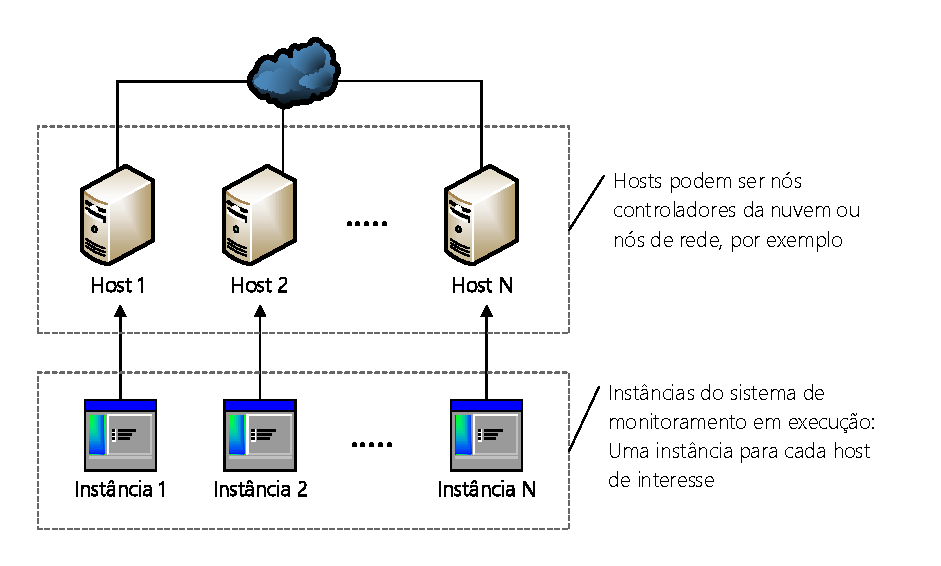
\includegraphics[width=.9\textwidth]{img/arquitetura_instalacao.pdf}
	\label{fig:proposta_instalacao}\\
    \vspace{-0.3cm}
	Fonte: O próprio autor.
\end{figure}

Apesar de nem todos os hosts hospedarem \acp{api} dos serviços (F2) ou o RabbitMQ (F3), pode haver interesse em monitorar tal host caso o tráfego de controle de algum serviço de interesse origine ou vá para ele (F1).
%
A decisão se o pacote está relacionado com algum serviço de interesse é baseada na porta de destino, seguindo as portas por padrão na Tabela \ref{tab:openstack_service_list}.
%
Para realizar a coleta de tráfego, este sistema de monitoramento será desenvolvido em uma linguagem de alto nível que forneça métodos relacionados à biblioteca \texttt{libpcap}.
%
Esta biblioteca disponibiliza meios para sistemas UNIX capturarem tráfego em suas interfaces de rede, sendo elas virtuais ou físicas.
%
Das linguagens possíveis, a preferência é para Python, por dispor de diversas bibliotecas e funcionalidades que simplificam o desenvolvimento, mas podendo mudar caso desempenho torne-se um fator crítico, seguindo o requisito RNF2.

Abordando o comportamento do sistema em alto nível é possível abstrair comportamentos comuns às três funcionalidades, conforme ilustrado na Figura~\ref{fig:proposta_funcionamento}.
%
\begin{figure}[!htb]
	\centering
	\caption{Arquitetura do sistema de monitoramento em alto nível}
    \vspace{-0.5cm}
	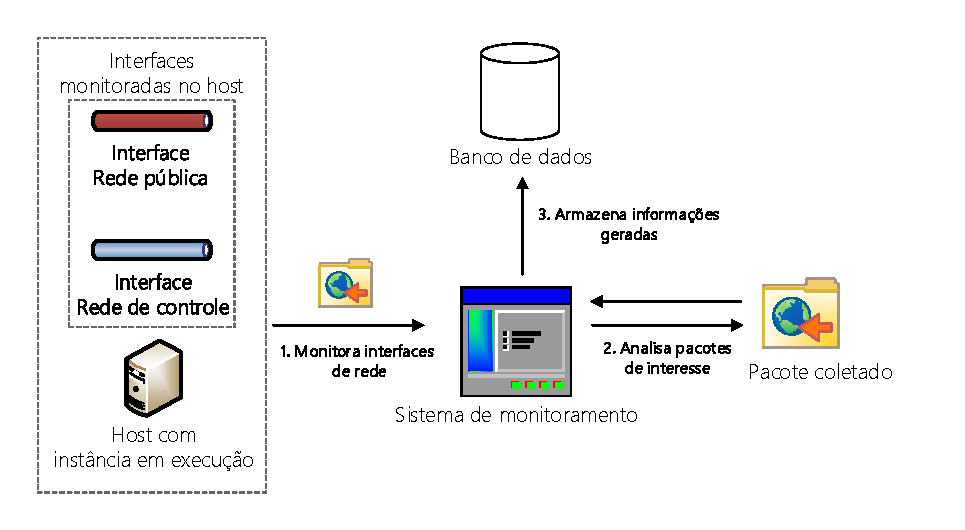
\includegraphics[width=1\textwidth]{img/arquitetura_funcionamento.pdf}
	\label{fig:proposta_funcionamento}\\
    \vspace{-0.6cm}
	Fonte: O próprio autor.
\end{figure}

\vspace{-0.3cm}
O sistema de monitoramento executará em um host de interesse, coletando tráfego nas interfaces de rede de acordo com as funcionalidades do sistema de monitoramento em execução naquele host, respeitando o requisito RNF1 (passo 1 na Figura \ref{fig:proposta_funcionamento}).
%
Caso um host não hospede \acp{api} de serviços, ou o \textit{middleware} de comunicação, por exemplo, é possível executar o sistema de monitoramento apenas para monitorar o tráfego na interface da rede de controle, pois é por onde passa o tráfego dos serviços de interesse, que é registrado pela F1.
%
Apesar de existirem outros níveis de agregação de tráfego, neste sistema de monitoramento é necessário realizar a medição a nível de pacote.
%
A agregação a nível de fluxo, por exemplo, apesar de popular, omite detalhes relevantes para este sistema de monitoramento, como o conteúdo do pacote.
%
Outro motivo é que apenas um pacote pode ser o suficiente para provocar mudanças no comportamento da nuvem, tal como uma requisição de criação de instância.
%
A agregação de tráfego com uma granularidade mais grossa perde tais detalhes, que devem ser levados em consideração no monitoramento, de acordo com o requisito RF4.

Os pacotes coletados são filtrados conforme a funcionalidade em execução no sistema de monitoramento daquele host, que nos três casos verificam a porta de destino (passo 2 na Figura \ref{fig:proposta_funcionamento}).
%
Na F1, qualquer pacote que tenha a porta de destino pertencente a uma das portas contida na Tabela \ref{tab:openstack_service_list}, por padrão, será aceito.
%
Em relação à F2, apenas pacotes destinados às portas na qual as \acp{api} executam serão aceitos.
%
Para a F3, os pacotes destinados à porta na qual o RabbitMQ executa serão aceitos.
%
Após, cada funcionalidade realiza seu processamento utilizado informações extraídas dos pacotes filtrados, posteriormente gravando no banco de dados escolhido, que é acessado por todas as instâncias em execução para gravar as informações geradas (passo 3 na Figura \ref{fig:proposta_funcionamento}).
%
Em relação aos dados armazenados, cada funcionalidade terá sua própria estrutura de armazenamento no banco de dados, que no caso de banco de dados relacionais (\textit{i.e.,} MySQL, PostgreSQL), é o equivalente a uma ou mais tabelas para cada funcionalidade.
%
O restante desta seção detalhará o funcionamento das três funcionalidades de monitoramento, na qual F2 e F3 serão agrupadas na explicação por conta da sua semelhança no funcionamento.

\subsection{F1: Classificação consumo de banda, rede de controle}
% @TODO -> parei revisão 1 aqui
Esta funcionalidade tem como objetivo auxiliar na análise longitudinal de tráfego na rede de controle.
%
Contudo, será considerado apenas o tráfego gerado pelos serviços delimitados na Tabela~\ref{tab:openstack_service_list} para simplificar o escopo deste TCC.
%
O diagrama de sequência na Figura \ref{fig:proposta_sequencia_servicos} ilustra os passos de funcionamento desta funcionalidade do sistema de monitoramento.

\begin{figure}[!htb]
	\centering
	\caption{Diagrama de sequência: monitoramento de banda consumida pelos serviços}
    \vspace{-0.3cm}
	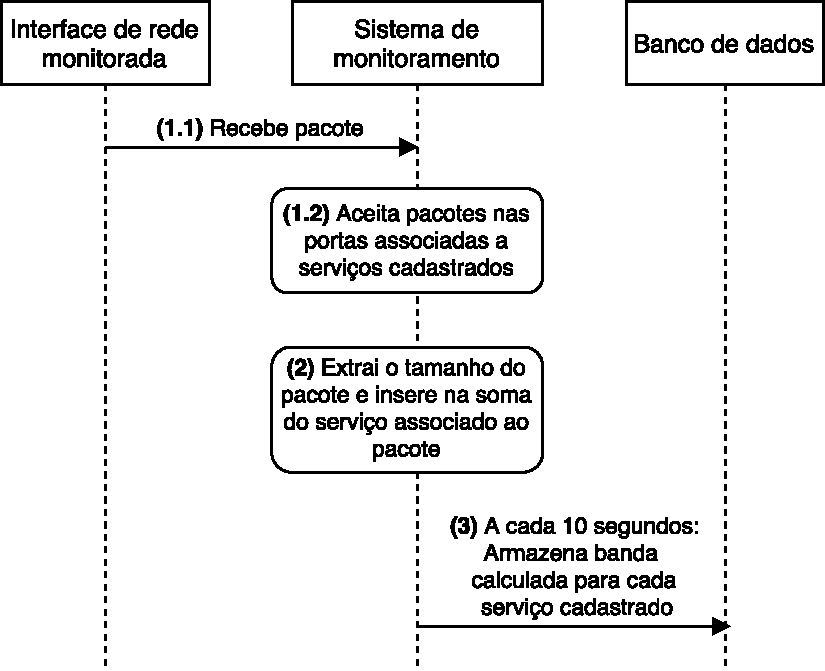
\includegraphics[width=0.77\textwidth]{img/sequencia_monitoramentoServicos.pdf}
	\label{fig:proposta_sequencia_servicos}\\
%    \vspace{-0.3cm}
	Fonte: O próprio autor.
\end{figure}

Os passos que esta funcionalidade executa são:

\begin{enumerate}
\item Esta funcionalidade monitora apenas a interface da rede de controle, buscando todo tráfego que tenha como destino uma das portas associadas aos serviços em execução naquele host.
%
As portas também são utilizadas para criar uma classificação de serviços, cuja porta de destino serve para decidir em qual serviço aquele pacote está associado;

\item Após definido o serviço destino daquele pacote, é extraído o tamanho daquele pacote, que é somado a um contador de tráfego para aquele serviço.
%
Assim, por exemplo, todos os pacotes recebidos por certo serviço ao longo de um tempo têm seu tamanho somado, e então esta soma é dividida pelo período de tempo estabelecido (\textit{e.g.,} 5s, 10s).
%
Ou seja, ao somar todo o tráfego recebido ao longo de um período, e depois dividir esta soma pelo período, é possível estabelecer uma aproximação da quantidade de banda utilizada (em KB/s) para o serviço em questão naquele período.
%
Esta técnica é feita para todos os serviços considerados nesta análise, cada qual tendo seu próprio contador; e

\item Para cada uma destas somas é feita uma entrada no banco de dados, contendo o serviço e o cálculo de banda usada pelo serviço.
%
No caso de oito serviços monitorados com um período de 10s, por exemplo, a cada 10s serão realizadas oito inserções, em que cada uma contém a quantidade de banda destinada ao seu serviço naqueles 10s.
%
Após realizada a inserção o contador de cada serviço volta para zero, e faz o processo de inserção no banco de dados após 10s novamente.
\end{enumerate}


\subsection{F2 e F3: Cadastrar eventos detectados na \ac{api} dos serviços e no \textit{middleware} de comunicação}

Ambas F2 e F3 comportam-se de maneira similar, variando apenas a porta de destino observada e o conteúdo/protocolo dos pacotes analisados.
%
A Figura~\ref{fig:proposta_sequencia_transacao} ilustra um diagrama de sequência para F3, que monitora as transações internas da nuvem passando pelo \textit{middleware} de comunicação.
%
Para gerar informações significativas deve-se relacionar os dados gerados por estas funcionalidades com outras, sendo possível relacionar as duas, por exemplo, e criar uma sequência detalhada de ações na nuvem a partir de uma requisição, conforme feito por \citeonline{sharma:2015:hansel}.

\begin{figure}[!htb]
	\centering
	\caption{Diagrama de sequência: monitoramento de transações internas da nuvem}
	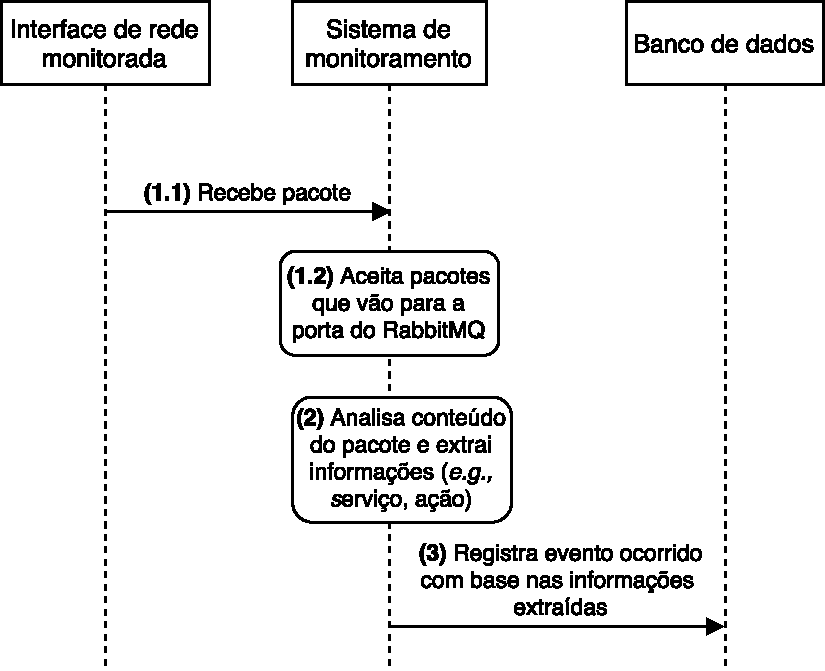
\includegraphics[width=0.78\textwidth]{img/sequencia_monitoramentoTarefas.pdf}
	\label{fig:proposta_sequencia_transacao}\\
	Fonte: O próprio autor.
\end{figure}

As ações nestas funcionalidades ocorrem da seguinte forma, tomando o diagrama de sequência da F3 (Figura \ref{fig:proposta_sequencia_transacao}) como base:

\begin{enumerate}
\item A F2 monitora a interface da rede pública, enquanto a F3 monitora a interface da rede de controle.
%
Ao receber pacotes, ambas as funcionalidades olham na porta de destino para decidir se aceitam os pacotes, na qual a F2 verifica se a porta de destino é de uma \ac{api} que o host hospeda; e no caso da F3, é verificado se a porta de destino é a mesma que a do \textit{middleware} de comunicação que o host hospeda; e

\item A princípio ambas as funcionalidades armazenarão as mesmas informações, mesmo que os protocolos de comunicação analisados sejam diferentes (HTTP na F2, e \ac{rpc} na F3).
%
Ou seja, para ambos as principais informações a armazenar são: serviço de origem, serviço de destino, IP do host e identificador da ação;

\item Por fim, armazena-se os dados de cada funcionalidade em suas respectivas tabelas.
\end{enumerate}


Conforme definido, através da implementação deste sistema de monitoramento será possível gerar os dados necessários para realizar a caracterização de tráfego proposta para a rede de controle.
%
A F1 é capaz de gerar informações relevantes em tempo real, possibilitando, por exemplo, verificar a variação do uso de banda pelos serviços ao longo de um período determinado.
%
Diferentemente, as funcionalidades F2 e F3 geram dados que necessitam de uma análise mais minuciosa, realizada na etapa posterior à coleta, especificada na Seção \ref{cap3:analise}.


\section{Análise de tráfego}
\label{cap3:analise}

A etapa de análise de tráfego, que será aplicada nos dados gerados pelo sistema de monitoramento (definido na Seção \ref{cap3:monitoramento}) busca gerar informações que ajudem a compreender melhor o comportamento do tráfego analisado.
%
Esta análise terá escopo limitado, no sentido de considerar apenas os serviços contidos na implementação mais popular de nuvem OpenStack, segundo \citeonline{openstack:newton}: Nova, Neutron, Cinder, Swift, Keystone e Glance.
%
A proposta atual pretende caracterizar três ângulos diferentes na rede de controle:

\begin{itemize}
	\item \textbf{Caracterização de funcionalidades da nuvem:} Busca entender como a execução de tarefas pelo consumidor influencia no funcionamento da rede de Controle da nuvem. 
	%
	A proposta inicial tem foco no ciclo de vida de \acp{vm} do OpenStack (\textit{e.g.,} criação de \ac{vm}, iniciação de \ac{vm}, pausar \ac{vm} em execução).
	
	\item \textbf{Consumo de banda por serviços:} Esta análise longitudinal tem como objetivo entender quais dos serviços considerados na análise mais geram tráfego na rede de Controle.
	
	\item \textbf{Influência de eventos periódicos no comportamento da nuvem:} Listar alguns dos eventos periódicos gerados pelos serviços da nuvem, e verificar qual o impacto gerado por eles na rede de controle. 
\end{itemize}

A \textbf{caracterização de funcionalidades da nuvem} utilizará informações geradas pelas F2 e F3, definidas no sistema de monitoramento.
%
Estas funcionalidades geram dados referentes à comunicação com as \acp{api} da nuvem, e da comunicação interna dos serviços, feita através do RabbitMQ.
%
Sendo assim, é possível criar uma sequência que mostra a trajetória do tráfego durante a realização de uma tarefa na nuvem a partir de uma requisição recebida pela \ac{api}.
%
Ou seja, a partir de uma requisição de um consumidor (\textit{e.g., } criação de \ac{vm}), cria-se um grafo direcionado que mostra quais mensagens foram enviadas para quais serviços à fim de concretizar a tarefa em questão.
%
Segundo \cite{sharma:2015:hansel} é possível gerar esta sequência de eventos, mas ainda não foi realizada uma análise profunda para verificar se realmente existe alguma variável que pode ser utilizada para interligar estas mensagens diretamente.

A análise de \textbf{consumo de banda por serviços} baseia-se na F1 do sistema de monitoramento, que contabiliza o tráfego gerado por cada um dos serviços considerados na análise.
%
A F1 do sistema de monitoramento deve gerar dados que podem ser interpretados diretamente, possibilitando a realização desta análise em tempo real.
%
Sendo assim, é possível por exemplo, acessar os dados gerados por esta funcionalidade definindo o período de início e de fim da análise, na qual gera um gráfico mostrando qual a porcentagem de tráfego destinado a cada serviço.

Por fim, a análise da \textbf{influência de eventos periódicos no comportamento da nuvem} deve se basear principalmente nos dados gerados pela F1 do sistema de monitoramento, na qual buscará grandes variações no recebimento de tráfego dos serviços em curtos períodos de tempo.
%
Baseando-se nestas variações serão consultados os dados gerados pelas F2 e F3 naquele período, que constará quais serviços enviaram as mensagens em questão.
%
Ou seja, como produto final este ângulo de caracterização busca mostrar quem executou aquele evento periódico, qual a tarefa em questão, e se há impacto significativo.
%
Definida a abordagem utilizada para a realização da caracterização de tráfego, o passo final é explicar como será realizado o experimento que aplicará a proposta definida neste capítulo.


\section{Plano de testes}
\label{cap3:experimento}

O plano de testes visa definir os experimentos a serem executados, os quais aplicarão a proposta de caracterização de tráfego.
%
A finalidade destes experimentos é validar o sistema de monitoramento desenvolvido e a abordagem para análise do tráfego.
%
No total serão realizados três experimentos, divididos em dois cenários diferentes, sendo que dois experimentos serão realizados em um dos cenários, e o outro cenário será usado no experimento restante.

\begin{itemize}
\item \textbf{Cenário 1:} Uma nuvem OpenStack com ambiente controlado, na qual toda interação com ela será originária dos experimentos executados; e

\item \textbf{Cenário 2:} Uma nuvem OpenStack em ambiente de produção, com consumidores utilizando-a.
\end{itemize}

Os experimentos visam verificar o funcionamento do sistema de monitoramento, e então analisar os dados gerados após a execução. 
%
Estes experimentos são:

\iffalse
\begin{itemize}
	\item \textbf{Experimento 1:} Visa verificar o funcionamento da função do sistema de monitoramento responsável por registrar o consumo de banda na rede de controle dos serviços do OpenStack, que será realizado no \textbf{cenário 1}.
    %
    O sistema de monitoramento executará apenas a função responsável por registrar o consumo de banda dos serviços, na qual o período de monitoramento será de um dia.
    %
    Durante este período, a nuvem em questão não receberá qualquer requisição originária de consumidor, e não hospedará nenhuma \ac{vm} em execução.
    %
    Os dados de consumo de banda gerados neste experimento serão armazenados e analisados, com o objetivo de estabelecer uma linha base de consumo de banda em nuvens OpenStack.
\end{itemize}
\fi

\begin{itemize}
	\item \textbf{Experimento 1:} Verificar o funcionamento do sistema de monitoramento, com o objetivo de avaliar a quantidade de dados gerados no monitoramento do \textbf{Cenário 1}.
    %
    O sistema de monitoramento utilizará todos as suas funcionalidades, na qual instâncias executarão em todos os hosts de interesse por um período de sete dias.
    %
    Durante este período, a nuvem deverá receber algumas requisições, que simularão atividades de consumidores, mas de forma esporádica.
    %
    Deste modo, será avaliada a quantidade de dados gerados, com o objetivo de verificar, por exemplo, se o banco de dados utilizado é adequado no caso de monitorar uma nuvem em ambiente de produção.
\end{itemize}

\begin{itemize}
	\item \textbf{Experimento 2:} Análise longitudinal do consumo de banda pelos serviços de uma nuvem em ambiente de produção (\textbf{Cenário 2}).
    %
    A função que registra o consumo de banda pelos serviços do OpenStack executará por um período de 30 dias.
    %
    Após, com os dados coletados será feita uma análise, com o objetivo de verificar a variação do consumo ao longo do período, identificando padrões de comportamento, por exemplo.
\end{itemize}

\begin{itemize}
	\item \textbf{Experimento 3:} Caracterização do comportamento da rede de controle em uma nuvem em ambiente de produção (\textbf{Cenário 2}).
    %
    O sistema de monitoramento utilizará todas as suas funcionalidades, na qual instâncias executarão em todos os hosts de interesse por um período de sete dias.
    %
    Ao longo deste período, a nuvem em questão será usada pelos consumidores e o sistema de monitoramento irá gerar dados sobre o uso.
    %
    Após, será feita uma caracterização de tráfego abordando dois ângulos de análise, definidos na Seção \ref{cap3:analise}: influência de eventos periódicos no comportamento da nuvem, e caracterização de funcionalidades da nuvem.
\end{itemize}

	Como comparativo, serão avaliados o tamanho do banco de dados nos experimentos 1 e 3, e verificar se há grande mudança na quantidade de dados gerados a partir do monitoramento.
    %
    Ambos os cenários utilizarão uma instalação similar do OpenStack, na qual os serviços caracterizados serão os mesmos.
    
    
\section{Considerações do Capítulo}
\label{cap3:consideracoes}

Este capítulo apresentou a proposta de caracterização de tráfego para uma nuvem computacional OpenStack.
%
A proposta baseia-se na análise da arquitetura de funcionamento de alguns serviços do OpenStack, o que possibilitou a definição de estratégias para utilizar no sistema de monitoramento, responsável pela primeira etapa: a medição de tráfego.
%
Foram definidos requisitos para a criação deste sistema de monitoramento, que abordam suas funcionalidades, e também pré requisitos, que devem ser considerados na construção dele.
%
O sistema de monitoramento em questão terá três funcionalidades que irão medir o tráfego e popular um banco de dados com as informações geradas a partir do tráfego avaliado.
%
Então, a etapa posterior, de análise de tráfego utilizará estas informações para melhor entender o comportamento da rede de controle sobre três ângulos de análise diferentes.
%
Após definir o que deve ser feito, a especificação do plano de testes determinou quais os experimentos que serão realizados, e também estabeleceu os cenários empregados nos experimentos.
\chapter{Considerações \& Trabalhos futuros}
\label{cap:conclusao}

% 1. Uma explicação informando de modo claro se atingiu ou não os objetivos estabelecidos (aqui pode-se ter também uma subdivisão entre objetivos gerais e objetivos específicos). Em cada caso devem ser explicados os motivos:
%     a. Caso tenha atingido os objetivos: informar os principais fatores que contribuíram para o sucesso, descrevendo-os de forma breve porém que não deixem dúvidas;
%     b. Caso não tenha atingido os objetivos: informar o quanto do objetivo foi atingido e citar os fatores que contribuíram para o insucesso, descrevendo-os de forma breve porém que não deixe dúvidas.
% 2. Descrever as principais considerações e conclusões que foram obtidas em decorrência da execução do trabalho. Aqui não deve ser repetido texto já existente no trabalho mas escrever as impressões dessas considerações e como elas contribuíram para a execução e atingir o objetivo;
% 3. Citar e descrever as principais dificuldades encontradas para execução do trabalho e projeto. Todo o trabalho desenvolvido significa uma evolução para o aluno, sendo que para chegar essa evolução o mesmo necessitou transpor uma série de obstáculos. Relatar os obstáculos e como superou (ou não superou)  ajuda a dignificar e mostrar o mérito do trabalho em si para o leitor/ avaliador. Também é uma contribuição, no sentido que uma vez expostos os problemas e soluções os leitores/avaliadores aprendem/conhecem formas de resolução ou de abordagem a tais problemas;
% 4. Comentar se ocorreram modificações durante a execução do trabalho no escopo definido na fase de Projeto e no que fora desenvolvido. Deve ser explicado o quê gerou essas modificações, fundamentando e justificando tais alterações.
% 5. Pode ser descrita a relação entre cronograma proposto e cronograma realizado no trabalho. Permitindo assim o leitor/avaliador aprender com as distorções/acertos indicados.
% 6. Descrever ou citar trabalhos futuros que podem ser feitos com base nesse trabalho desenvolvido. No decorrer da execução de um trabalho busca-se atingir um objetivo definido no projeto, porém vários assuntos interessantes de pesquisar são  revelados (sendo que os mesmo não são tratados/pesquisados no trabalho por não condizerem com os objetivos / escopo do trabalho). A descrição de tais assuntos/temas/pesquisas demonstra a percepção desenvolvida pelo aluno no desenvolvimento assim como a sua visão de objetividade na execução desse trabalho.



Os jogos \ac{mmorpg} são utilizados como negócio viável e lucrativo, sendo que, a experiência de jogabilidade na qual o usuário final será submetido é um fator crítico para o sucesso destes jogos.
%
Tais serviços são implementados sobre arquiteturas que executam o serviço sobre diversos servidores, na qual o desempenho deste serviço e o custo de sua manutenção é um fator crítico para o sucesso de um jogo deste gênero.
%
Modelar um sistema de alto desempenho para tais serviços torna-se um trabalho essencial para a satisfação do usuário final neste cenário.


O atual trabalho teve como objetivo analisar as arquiteturas de microsserviços Rudy, Salz e Willson, caracterizadas especificamente para jogos \ac{mmorpg} com o objetivo de oferecer relações e efeitos sobre as arquiteturas selecionadas.
%
Esta análise é baseada na coleta de informações do consumo de recursos para sua execução e um valor de qualidade das arquiteturas, do ponto de vista do cliente.

Nesse sentido, o atual trabalho obteve sucesso ao realizar esta análise, gerando informação sobre uma relação entre a qualidade das arquiteturas de microsserviços selecionadas para um conjunto de regras de negócio de um jogo genérico e o consumo de recursos computacionais para as respectivas execuções.
%
Ambas as arquiteturas desempenharam seus papéis sem problemas, demonstrando características únicas na qual evidenciaram-se neste trabalho.

Um objetivo específico deste trabalho é validar as características obtidas da literatura, haja visto que os autores citavam o seu comportamento sem a comprovação destes comportamentos.
%
Dessa forma, o atual trabalho concluiu com sucesso a validação destas características, tornando tais dados como verdadeiros para futuros pesquisadores.

Outro fator pertinente após a análise é com relação ao gargalo encontrado, no qual mostrou-se relacionado a forma de obter e armazenar dados.
%
Entretanto, tal informação não é uma contribuição inicial do atual trabalho visto que outros autores do levantamento teórico realizado já citavam tal característica.

O atual trabalho concluiu que o desempenho, do ponto de vista de tempo de resposta, está relacionado a melhor utilização da \ac{cpu}, seja pelos microsserviços de armazenamento de dados ou por microsserviços de processamento de dados.
%
Mostrou-se viável a aplicação de sistemas de filas ou barreiras para gerenciamento do acesso ou minimização do consumo de um serviço interno, impactando diretamente na vazão dos dados pela arquitetura.
%
Outro critério de atenção é a sincronização de dados, a qual pode consumir um valor significativo de \ac{cpu} e, caso desempenhe um papel incompatível com o necessário, pode prejudicar o processamento e vazão dos dados pela arquitetura.

% Ao final deste trabalho, não foi possível analisar todos os dados obtidos.
%
A partir dos dados coletados, existem dados intermediários que não foram utilizados nesta análise.
%
Este conjunto de dados possui informações de monitoramento de todas as máquinas envolvidas nos experimentos de forma individual, quanto dos processos individuais na arquitetura do Docker Swarm e Docker Compose.
%
Pretende-se analisar esses dados, preferencialmente, durante a escrita de um artigo técnico científico previsto como trabalho futuro.

Este trabalho teve algumas dificuldades durante a sua execução.
%
Durante o processo de busca por referências teóricas na literatura, mostrou-se uma área atacada por diversos modelos para processamento de dados e desenvolvimento web.
%
Porém existe uma baixa frequência de publicações de artigos para jogos \ac{mmorpg}, abordando sua arquitetura em baixo nível.
%
Tal problema foi solucionado ao buscar as arquiteturas para jogos \ac{mmorpg} e encontrar modelos próximos em desenvolvimento web.

Outro problema significativo tem relação com a arquitetura e organização de código que foi necessário para a implementação das arquiteturas e clientes.
%
Por se tratar de um projeto de considerável porte, na qual teve a duração de seis meses de desenvolvimento, foram encontrados diversos problemas de engenharia de software para permitir o isolamento da regra de negócio de forma abstrata, garantindo que todas as arquiteturas estavam processando as requisições sem otimizações particulares.
%
Este problema foi superado ao utilizar técnicas de \textit{Clean Architecture} e testes automatizados utilizando uma suíte de integração contínua.
%
Estas técnicas aumentaram a produtividade para o desenvolvimento em longo prazo, permitindo a sua implementação em um menor espaço de tempo.
%

Uma dificuldade encontrada relaciona-se a infraestrutura dos ambientes, especificamente na limitação de recursos para a execução do experimento por completo na nuvem LabP2D.
%
Este problema foi resolvido migrando a estrutura dos clientes para um laboratório de computadores.
%
Durante esta migração, foi necessário a liberação de acesso a portas entre a nuvem e a rede do laboratório.
%
Por fim este problema foi resolvido junto ao suporte técnico da rede, permitindo a elaboração do atual trabalho.

A execução do atual trabalho não obteve alterações em seu escopo, entretanto foi executada em um período prolongado comparado ao estimado.
%
Tal prolongamento de execução do trabalho tem relação aos problemas citados anteriormente.

\section{Contribuições do TCC}

Este TCC contribui com futuros jogos \ac{mmorpg} ou arquiteturas distribuídas de outras áreas, a qual beneficiam-se dos dados, características e conclusões encontradas no atual trabalho.
%
Além desta contribuição, o atual trabalho também serve como guia de engenharia de software para a implementação de protótipos funcionais, contribuindo com exemplos designados a esta área na qual obteve-se dificuldades de encontrar material científico.

O atual trabalho também, indiretamente, contribuiu com diversas ferramentas e softwares \textit{OpenSource} durante o processo de implementação das arquiteturas, pois tais ferramentas necessitaram de pequenos ajustes para funcionamento de protocolos de redes.
%
A fim de criar um serviço válido, protótipos de clientes reais com o motor gráfico Godot foram implementados para validação do protocolo de comunicação do serviço.
%
A ferramenta que mais obteve contribuições foi o motor gráfico Godot, a qual recebeu diversas alterações em sua classe de conexão \ac{tcp} para viabilizar protótipos deste trabalho.
%
Tais alterações foram disponibilizadas no repositório oficial da ferramenta, sendo essa disponibilização aplicada a versão mais recente (3.1, disponível no segundo semestre de 2019) e consequentemente utilizadas por outros desenvolvedores da comunidade para desenvolvimento de futuros jogos.


O atual trabalho elabora resultados na qual pode suprir um tema pouco abordado nas pesquisas envolvendo arquiteturas de microsserviços.
%
Dessa forma, o atual trabalho contribui com futuras publicações sobre microsserviços e jogos \ac{mmorpg}.

\section{Trabalhos futuros}

Este TCC permite uma sequência de trabalhos futuros.
%
Alguns possíveis trabalhos futuros podem utilizar os dados pertinentes neste trabalho, tal qual analisar o impacto de melhorias ou otimizações em tais sistemas.
%
Também pode-se abordar os temas adjacentes utilizados neste trabalho, como tecnologias, protocolos ou metodologias utilizadas no desenvolvimento, implantação e análise do atual trabalho, utilizando os resultados e ferramentas desenvolvidas em futuras pesquisas.
%
Em específico, pode-se continuar este trabalho com os seguintes sugestões de temas:

\begin{itemize}
 \item Predição do uso de recursos baseado no modelo computacional das arquiteturas Rudy, Salz e Willson;
 \item Análise do gerenciador de processos do Docker na validação de consumo de \ac{cpu} com características senoidais;
 \item Análise do impacto na troca do ambiente de implantação;
 \item Análise do impacto no tempo de resposta ao remover o sistema de monitoramento de uso de recursos;
 \item Análise do impacto no troca dos serviços de bando de dados;
 \item Análise do impacto na utilização do sistema de assinatura de dados \ac{jwt} como sistema de autorização;
 \item Análise do impacto na otimização dos protocolos de comunicação utilizados;
 \item Anaĺise do consumo de recursos pela arquitetura de armazenamento de métricas; e
 \item Análise dos dados capturados mas não analisados no atual trabalho.
\end{itemize}

Além destes temas para contribuiões futuras, pretende-se publicar artigos com resultados obtidos no atual trabalho.
%
Dessa forma, pretende-se contribuir na linha de pesquisa de sistemas distribuídos, específicos sobre os temas de microsserviços e serviços para jogos \ac{mmorpg}.


%\section*{Agradecimentos}

AGRADECIMENTOS


%---------- Referências ------------------------------------
\renewcommand{\bibname}{Referências}
\bibliographystyle{pkg/abnt-alf}
\bibliography{refsTcc}

%---------- Apêndice ---------------------------------------
%\appendix
%\chapter{Apêndice: Cronograma}
\label{ap:crono}

%Até o presente momento, o cronograma proposto no Plano de \ac{TCC} está sendo realizado conforme o definido, na ordem e nos prazos estipulados. 

As seguintes etapas definidas no Plano de \ac{TCC} são as etapas já concluídas ou que serão realizadas para atingir os objetivos propostos:

	






%-----------------------------------------------------------
\end{document}
